\section*{9. TASK 2 IMPLEMENTATION}

\phantomsection
\addcontentsline{toc}{section}{9. TASK 2 IMPLEMENTATION}

For Task 2 we built a working prototype of the part of the factory application that sits closest to the gate. It covers M1 Gate Core, which handles a QR scan from the kiosk until the gate is closed again (Flow A), and M3 Gate Intervention, which lets a guard open a lane by hand or release it in an emergency (Flow B). This chapter first explains what is in the prototype and how the code is organized, then follows one scan through the code, and ends with the tests and their results.

\Needspace{9\baselineskip}
\subsection*{9.1. Scope of the Prototype}

\phantomsection
\addcontentsline{toc}{subsection}{9.1. Scope of the Prototype}

We picked Gate Core because most of the hard rules of the design meet there: the 2-second answer to the kiosk, the single-use QR claim, the order of opening, passage, and closing, and degraded mode (Sections 4.2.2 and 5.7.2). Gate Intervention is small, but it is the second user of the Gate Core interfaces, so it shows whether those interfaces were split well. Table 9.1 lists which parts are real code, which parts only exist to make the demo possible, and which parts we left out.

\begin{longtable}{|>{\raggedright\arraybackslash}p{110.5pt}|>{\raggedright\arraybackslash}p{80.5pt}|>{\raggedright\arraybackslash}p{219.5pt}|}
\hline
\multicolumn{1}{|>{\columncolor{tableheader}\centering\arraybackslash}p{110.5pt}|}{\textbf{Part}} & \multicolumn{1}{>{\columncolor{tableheader}\centering\arraybackslash}p{80.5pt}|}{\textbf{Status}} & \multicolumn{1}{>{\columncolor{tableheader}\centering\arraybackslash}p{219.5pt}|}{\textbf{What the code does}} \\
\hline
\endhead
\multicolumn{3}{c}{\rule{0pt}{20pt}\normalsize\textbf{Table 9.1. Scope of the Task 2 Prototype}} \\
\endlastfoot
M1 Gate Core & Implemented & Access check against the factory snapshot, the atomic write of ACCEPTED, TokenReservation, and GateCycle before openGate, PASSAGE and LANE\_CLEAR handling, attendance only after a stored passage, the 15-second passage timeout driven by a background worker, degraded mode, and the Gate Core side of assisted and emergency opening, where an emergency takes priority over an open result that arrives late. \\
\hline
M3 Gate Intervention & Implemented & Guard identity from the session, server-side authority check, write-once support cases, assisted opening, emergency release, and emergency reset. \\
\hline
Factory storage (SQLite) & Implemented & SqliteUnitOfWork and the SQLite repositories behind the storage ports of Gate Core: the atomic accept write, the token claim per factory, passage and attendance in one transaction, the outbox, event deduplication, and the eligibility snapshot, which is stored in the same transaction as its deduplication mark. \\
\hline
M2 Turnstile Adapter & Simulated & SimulatedTurnstileAdapter and FaultyTurnstileAdapter implement the turnstile ports against a simulated controller. Both pass the same contract tests, and SimulatedTurnstileAdapter also answers status queries. No real controller is connected. \\
\hline
QR issuer (part of M4) & Demo helper only & Signs 60-second Ed25519 tokens inside the same process so the demo can produce valid codes. In the target design this runs in the central application. \\
\hline
Controller simulator & Demo helper only & Swagger endpoints that play the controller: they send PASSAGE and LANE\_CLEAR and choose the simulated command results. \\
\hline
Audit, Monitoring, Identity \& RBAC & Stubs & In-memory stubs behind IAuditApi, IHealthApi, IAuthorizationApi, and IGuardIdentityApi. \\*
\hline\noalign{\nobreak}
Not implemented & -- & Station Client UI, Site Sync over the WAN, the central application, Attendance Consolidation and Review, HR/Payroll Handover, the standby server, and any real turnstile or broker. \\
\hline
\end{longtable}
\phantomsection\addcontentsline{lot}{table}{\protect\numberline{9.1}Scope of the Task 2 Prototype}

Since there is no real controller, central application, or standby server, the prototype says nothing about failover, WAN recovery, or the response time on factory hardware. What it can show is that the module boundaries and the gate rules from Chapters 4 to 7 can be written down in code and tested. Section 9.8 comes back to these limits.

\Needspace{9\baselineskip}
\subsection*{9.2. Technology Stack and Repository}

\phantomsection
\addcontentsline{toc}{subsection}{9.2. Technology Stack and Repository}

The code, the tests, and the source of this report are kept in one GitHub repository, described in Section 9.9. Table 9.2 shows the tools we used and why each one fits this prototype.

\begin{longtable}{|>{\raggedright\arraybackslash}p{90.5pt}|>{\raggedright\arraybackslash}p{120.5pt}|>{\raggedright\arraybackslash}p{199.5pt}|}
\hline
\multicolumn{1}{|>{\columncolor{tableheader}\centering\arraybackslash}p{90.5pt}|}{\textbf{Concern}} & \multicolumn{1}{>{\columncolor{tableheader}\centering\arraybackslash}p{120.5pt}|}{\textbf{Choice}} & \multicolumn{1}{>{\columncolor{tableheader}\centering\arraybackslash}p{199.5pt}|}{\textbf{Reason}} \\
\hline
\endhead
\multicolumn{3}{c}{\rule{0pt}{20pt}\normalsize\textbf{Table 9.2. Technology Stack of the Prototype}} \\
\endlastfoot
Language & Python 3.12 & Every member could read and review it, and abstract base classes are enough to express the ports. \\
\hline
Web API and demo & FastAPI with Uvicorn & Swagger UI at \code{/docs} lets us run Flow A and Flow B by hand without writing a client. \\
\hline
Factory storage & SQLite (\texttt{sqlite3}) & A single file database is enough for one factory application in a demo, and it supports the transactions that IUnitOfWork needs. It stands in for the factory database of Chapter 5, not for the replicated pair. \\
\hline
QR signatures & \texttt{cryptography}, Ed25519 & Matches ADR-11: the issuer holds the private key, and the factory only holds public keys in its snapshot. \\
\hline
Tests & pytest, FastAPI TestClient (httpx) & Unit, rule, HTTP, and architecture tests in one runner. \\*
\hline\noalign{\nobreak}
CI and packaging & GitHub Actions, Dockerfile & CI runs the full test suite on every push and pull request to \texttt{main} and \texttt{dev}. The Dockerfile starts the API on port 8000. \\
\hline
\end{longtable}
\phantomsection\addcontentsline{lot}{table}{\protect\numberline{9.2}Technology Stack of the Prototype}

To run the tests and the demo from the repository root:

\begin{itemize}[leftmargin=36pt, itemsep=2pt, topsep=4pt, parsep=2pt]
  \item \texttt{pip install -r requirements.txt}
  \item \texttt{PYTHONPATH=src pytest}
  \item \texttt{PYTHONPATH=src uvicorn tmc\_gate.api.app:app} (data in memory), or with \texttt{TMC\_GATE\_DB=factory.sqlite3} set first to keep the data in a SQLite file across restarts
  \item open \code{http://localhost:8000/docs} in a browser
\end{itemize}

\Needspace{9\baselineskip}
\subsection*{9.3. Code Structure}

\phantomsection
\addcontentsline{toc}{subsection}{9.3. Code Structure}

The code lives in one Python package, \code{src/tmc_gate}. We describe it in four steps: the folders and their import rules, how the design names map to files, the tables in the factory database, and the HTTP endpoints.

\Needspace{9\baselineskip}
\subsubsection*{9.3.1. Folders and Layers}

\phantomsection
\addcontentsline{toc}{subsubsection}{9.3.1. Folders and Layers}

The folders follow the Entry, Business, and Persistence layers of Gate Core in Figure 4.2 (Section 4.1.6). The interfaces that Gate Core owns have their own folder, \code{ports/}, between the business rules and the adapters, so the business code can depend on them without knowing which adapter is behind them. Table 9.3 shows what each folder holds and what it is allowed to import. The last column separates imports between our own folders from external libraries: the import tests only forbid the application layer from using storage, web, and adapter code, so AccessDecision may use the \texttt{cryptography} library directly to verify the Ed25519 signature. We did not want this to stay a convention that people could forget, so \code{tests/test_architecture_solid.py} reads the import statements of every file and fails when a layer imports something it should not.

\begin{longtable}{|>{\raggedright\arraybackslash}p{86.5pt}|>{\raggedright\arraybackslash}p{194.5pt}|>{\raggedright\arraybackslash}p{129.5pt}|}
\hline
\multicolumn{1}{|>{\columncolor{tableheader}\centering\arraybackslash}p{86.5pt}|}{\textbf{Folder}} & \multicolumn{1}{>{\columncolor{tableheader}\centering\arraybackslash}p{194.5pt}|}{\textbf{Contents}} & \multicolumn{1}{>{\columncolor{tableheader}\centering\arraybackslash}p{129.5pt}|}{\textbf{May import}} \\
\hline
\endhead
\multicolumn{3}{c}{\rule{0pt}{20pt}\normalsize\textbf{Table 9.3. Folders of the Task 2 Code}} \\
\endlastfoot
\code{domain/} & Entities and states of Section 4.3 and Tables 4.23a--b: Lane, ScanAttempt, TokenReservation, GateCycle, GateCommand, PassageEvent, AttendanceTransaction, SupportCase, and EligibilitySnapshot with the 60-second and 30-minute limits. & Nothing outside \code{domain/} \\
\hline
\code{ports/} & Interfaces owned by Gate Core: IScanSubmission, IInterventionRequest, IFactoryUpdates, the turnstile ports, IUnitOfWork, the repository ports, IPassageWindowQuery, and the cross-cutting ports. & \code{domain/} \\
\hline
\code{application/} & AccessDecision, GateTransactionProcessor, GateCoreFacade, InterventionService, and GateInterventionFacade. & \code{domain/}, \code{ports/}; external library: \texttt{cryptography} (Ed25519 check in AccessDecision) \\
\hline
\code{adapters/} & SQLite repositories and unit of work, PassageTimeoutWorker, the simulated turnstile adapters, the demo QR issuer, the demo guard sessions, and in-memory stubs. & All inner layers; external libraries: \texttt{sqlite3}, \texttt{cryptography} \\*
\hline\noalign{\nobreak}
\code{api/} & FastAPI routers for the kiosk, the controller signals, the guard actions, and the demo helpers. \code{app.py} is the composition root that creates every object and passes the adapters in. & Everything \\
\hline
\end{longtable}
\phantomsection\addcontentsline{lot}{table}{\protect\numberline{9.3}Folders of the Task 2 Code}

Figure 9.1 puts the same folders together with the parts outside the code. Everything inside \code{src/tmc_gate} runs in one Python process, including the simulated controller. That controller is ControllerApiClient in \code{adapters/turnstile_adapter.py}: it answers openGate, closeGate, the emergency commands, and status queries, but it never sends PASSAGE or LANE\_CLEAR by itself. In the demo runs these two signals are sent to the signal routes by the demo script or from Swagger UI, and in the tests by the test code, each time playing the controller. The four callers at the top reach only the \code{api/} routers. The kiosk scan routes hold IScanSubmission and the signal routes hold IPassageEvents. The guard router holds GateInterventionFacade, the public class of M3, together with IGuardIdentityApi for the session check. The demo router is wired with the demo QR issuer, the snapshot and attendance repositories, and ControllerApiClient, and it only exists in demo mode. In the application layer, GateCoreFacade and GateTransactionProcessor both implement ports and use other ports: the facade implements the three inbound ports and uses the repository ports, and the processor implements IPassageEvents and uses the command, repository, and cross-cutting ports. The SQLite file is only touched by \code{sqlite_repos}.

\noindent\begin{minipage}{\linewidth}
\centering
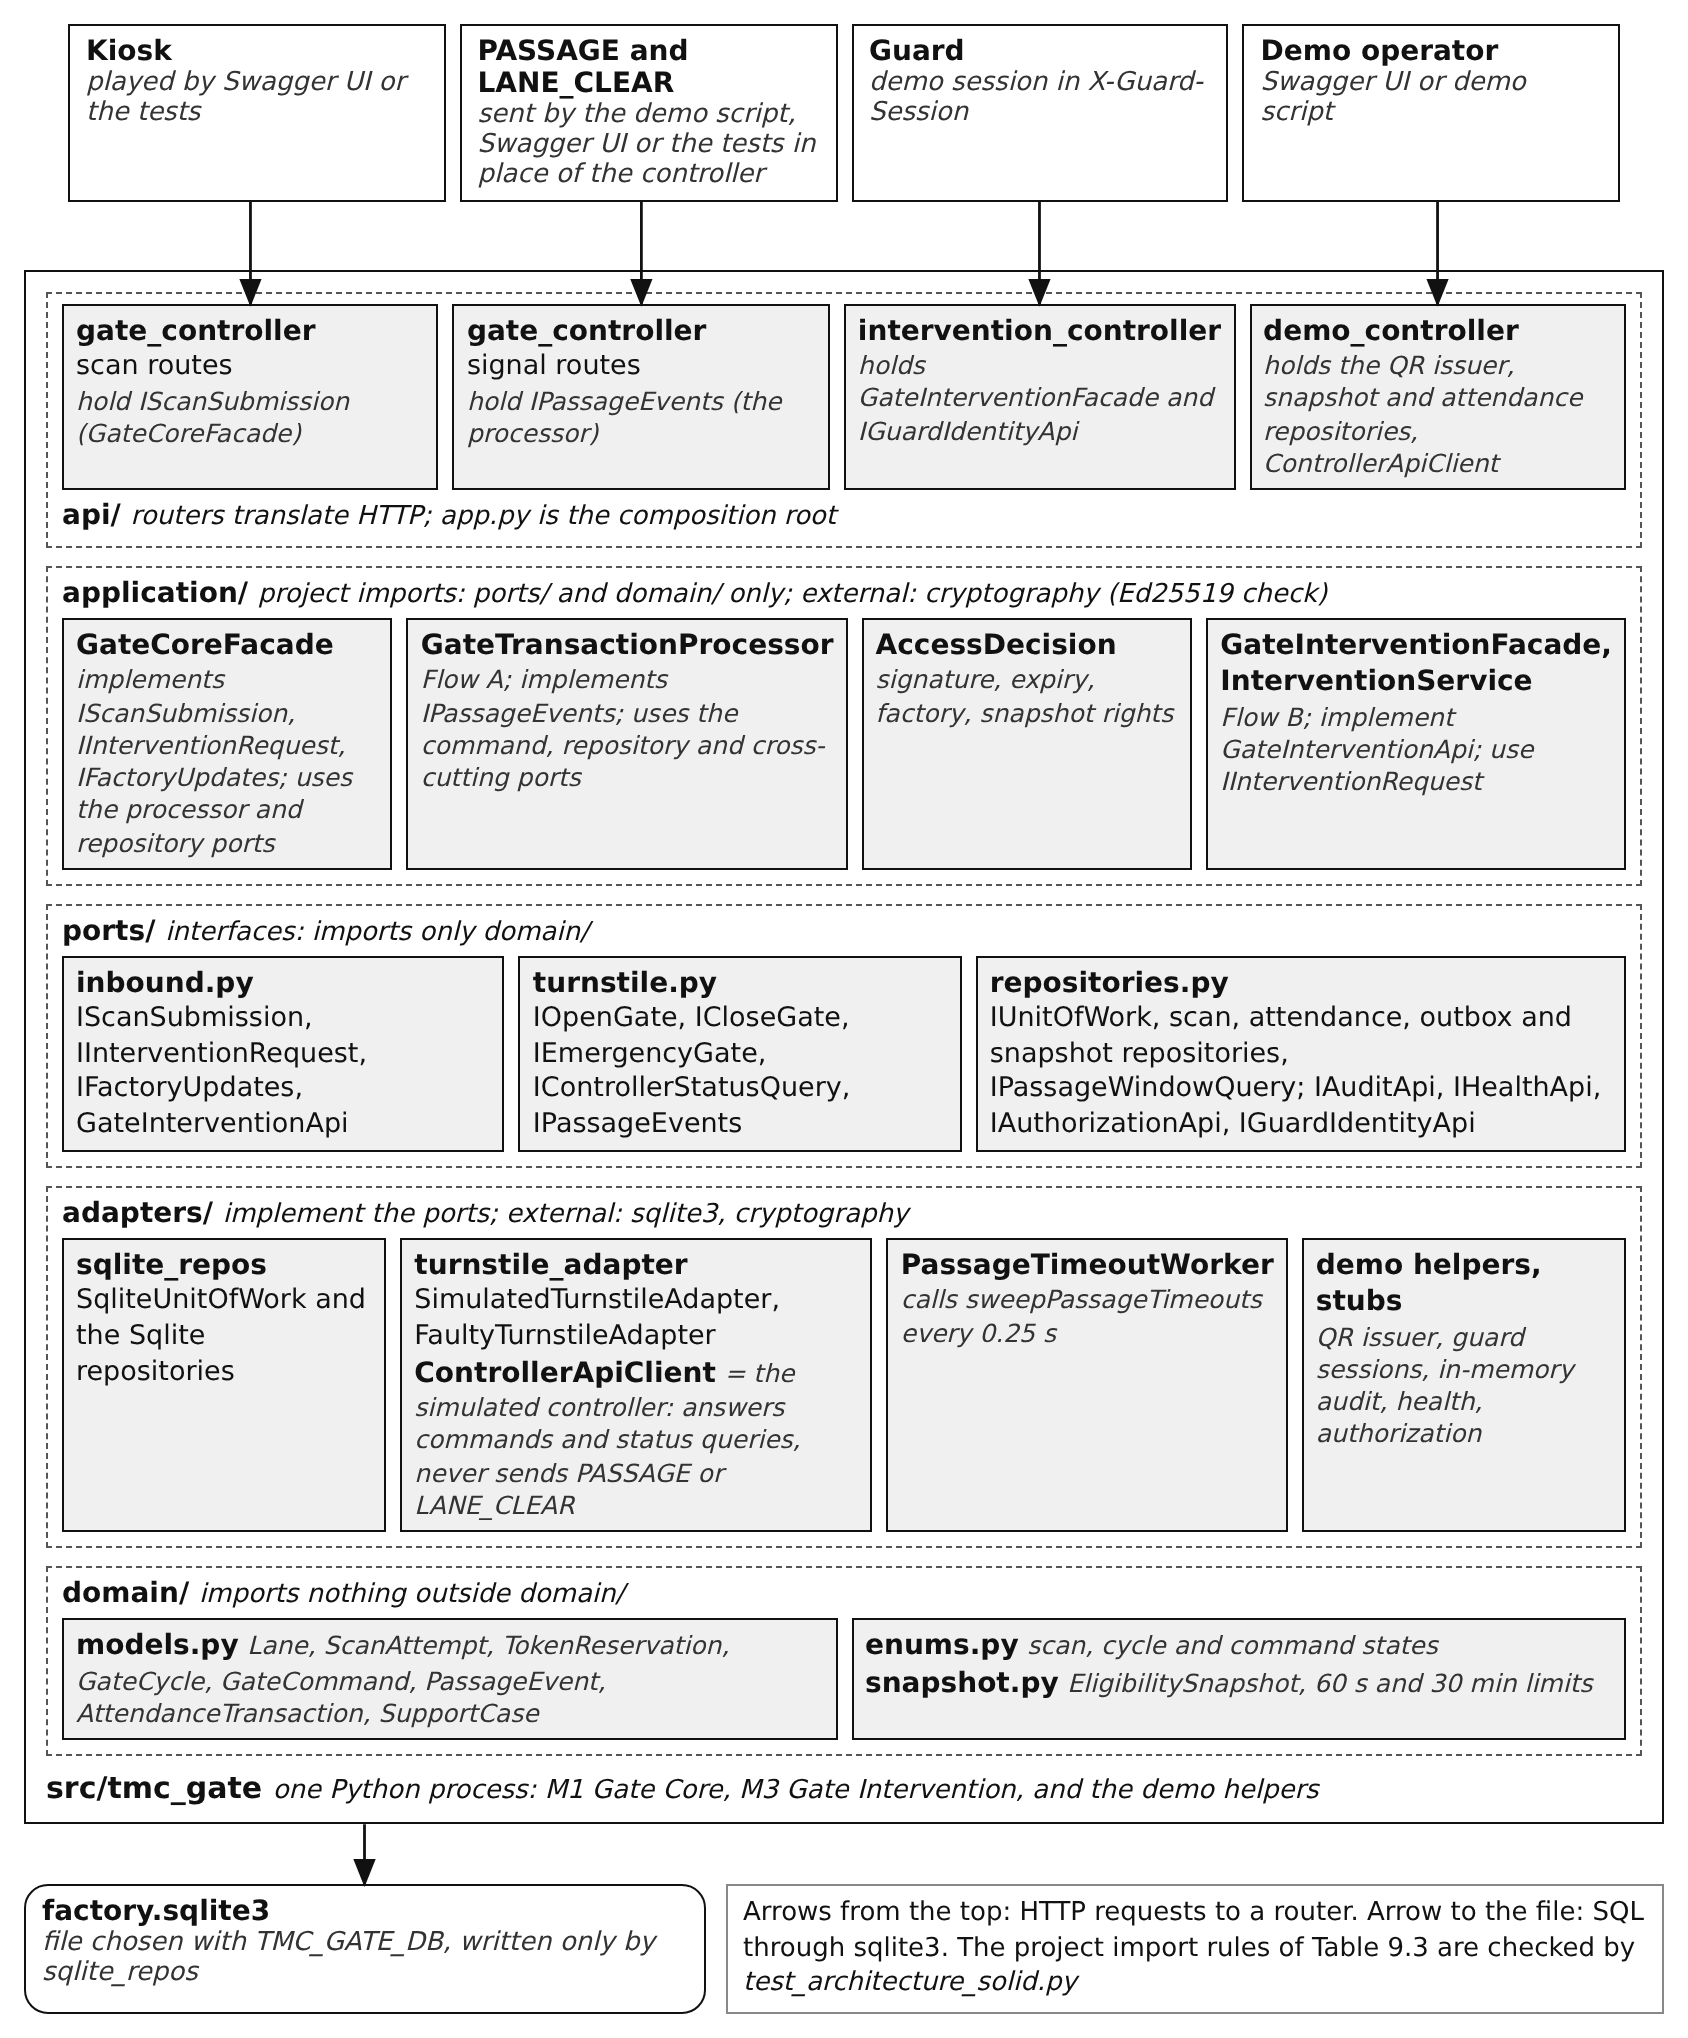
\includegraphics[width=0.98\linewidth]{diagram/implementation/figure-9-1-prototype-structure.png}

\vspace{6pt}
\textbf{Figure 9.1. Internal Structure of the Task 2 Prototype}
\phantomsection\addcontentsline{lof}{figure}{\protect\numberline{9.1}Internal Structure of the Task 2 Prototype}
\end{minipage}

\vspace{10pt}

\Needspace{9\baselineskip}
\subsubsection*{9.3.2. From the Design to the Code}

\phantomsection
\addcontentsline{toc}{subsubsection}{9.3.2. From the Design to the Code}

We tried to keep the names of Chapter 4 in the code, so a reader can take a component from a table or a figure and find it in a file. Table 9.4 lists the main pairs.

\begin{longtable}{|>{\raggedright\arraybackslash}p{150.5pt}|>{\raggedright\arraybackslash}p{260.5pt}|}
\hline
\multicolumn{1}{|>{\columncolor{tableheader}\centering\arraybackslash}p{150.5pt}|}{\textbf{Design element}} & \multicolumn{1}{>{\columncolor{tableheader}\centering\arraybackslash}p{260.5pt}|}{\textbf{Where it is in the code}} \\
\hline
\endhead
\multicolumn{2}{c}{\rule{0pt}{20pt}\normalsize\textbf{Table 9.4. Mapping from the Design to the Code}} \\
\endlastfoot
GateCoreController (Table 4.7) & \code{api/gate_controller.py} for the HTTP routes and GateCoreFacade in \code{application/facade.py}, which implements GateCoreApi \\
\hline
ControllerSignalHandler (Table 4.7) & The two signal routes in \code{api/gate_controller.py}; they call onPassage and onLaneClear of GateTransactionProcessor through IPassageEvents \\
\hline
GateTransactionProcessor (Table 4.7) & \code{application/processor.py} \\
\hline
AccessDecision, EligibilitySnapshot (Table 4.7) & \code{application/access_decision.py}, \code{domain/snapshot.py} \\
\hline
ScanRepo, AttendanceRepo, OutboxRepo (Table 4.7) & Ports in \code{ports/repositories.py}; SqliteScanRepository, SqliteAttendanceRepository, SqliteOutboxRepository, and SqliteUnitOfWork in \code{adapters/sqlite_repos.py} \\
\hline
GateInterventionController, Facade, InterventionService (Table 4.9) & \code{api/intervention_controller.py}; InterventionService and GateInterventionFacade in \code{application/intervention.py} \\
\hline
TurnstileAdapter, ControllerApiClient (Table 4.8) & SimulatedTurnstileAdapter, FaultyTurnstileAdapter, and ControllerApiClient in \code{adapters/turnstile_adapter.py} \\
\hline
GateCoreApi and the turnstile ports (Table 4.20) & \code{ports/inbound.py} (IScanSubmission, IInterventionRequest, IFactoryUpdates) and \code{ports/turnstile.py} (IOpenGate, ICloseGate, IEmergencyGate, IPassageEvents, IControllerStatusQuery) \\
\hline
Entities and states (Figure 4.20, Tables 4.23a--b) & \code{domain/models.py} and \code{domain/enums.py} \\
\hline
15-second passage window (Table 4.23b) & PassageTimeoutWorker in \code{adapters/passage_timeout_worker.py}, which calls GateTransactionProcessor.sweepPassageTimeouts \\*
\hline\noalign{\nobreak}
QR credential issuance in M4 (ADR-11) & QrCredentialIssuance in \code{adapters/demo_qr_issuer.py}, a demo stand-in for the central issuer \\
\hline
\end{longtable}
\phantomsection\addcontentsline{lot}{table}{\protect\numberline{9.4}Mapping from the Design to the Code}

Two names do not appear as classes. GateCoreController became a thin FastAPI router plus GateCoreFacade, because the router should only translate HTTP and the facade is what other modules see. ControllerSignalHandler became two routes that call the processor directly, since a separate class would only forward the call. StationClient, the kiosk application of the target design, is not built at all; Swagger UI and the tests play its role. The class diagrams in Figures 4.18 to 4.20 were drawn from this code, so they use the same names as Table 9.4.

\Needspace{9\baselineskip}
\subsubsection*{9.3.3. Factory Database}

\phantomsection
\addcontentsline{toc}{subsubsection}{9.3.3. Factory Database}

Figure 9.2 shows the tables that the SQLite adapters create in the factory database file, which is chosen with the \texttt{TMC\_GATE\_DB} variable. Each gate record has its own table. Next to them are the outbox, the marks used to drop repeated incoming events, the local audit evidence, and the last applied eligibility snapshot. EmployeeRight does not get a table of its own; its values are kept inside \code{eligibility_snapshots.snapshot_json}.

\noindent\begin{minipage}{\linewidth}
\centering
\IfFileExists{diagram/data/figure-9-2-data-view.png}{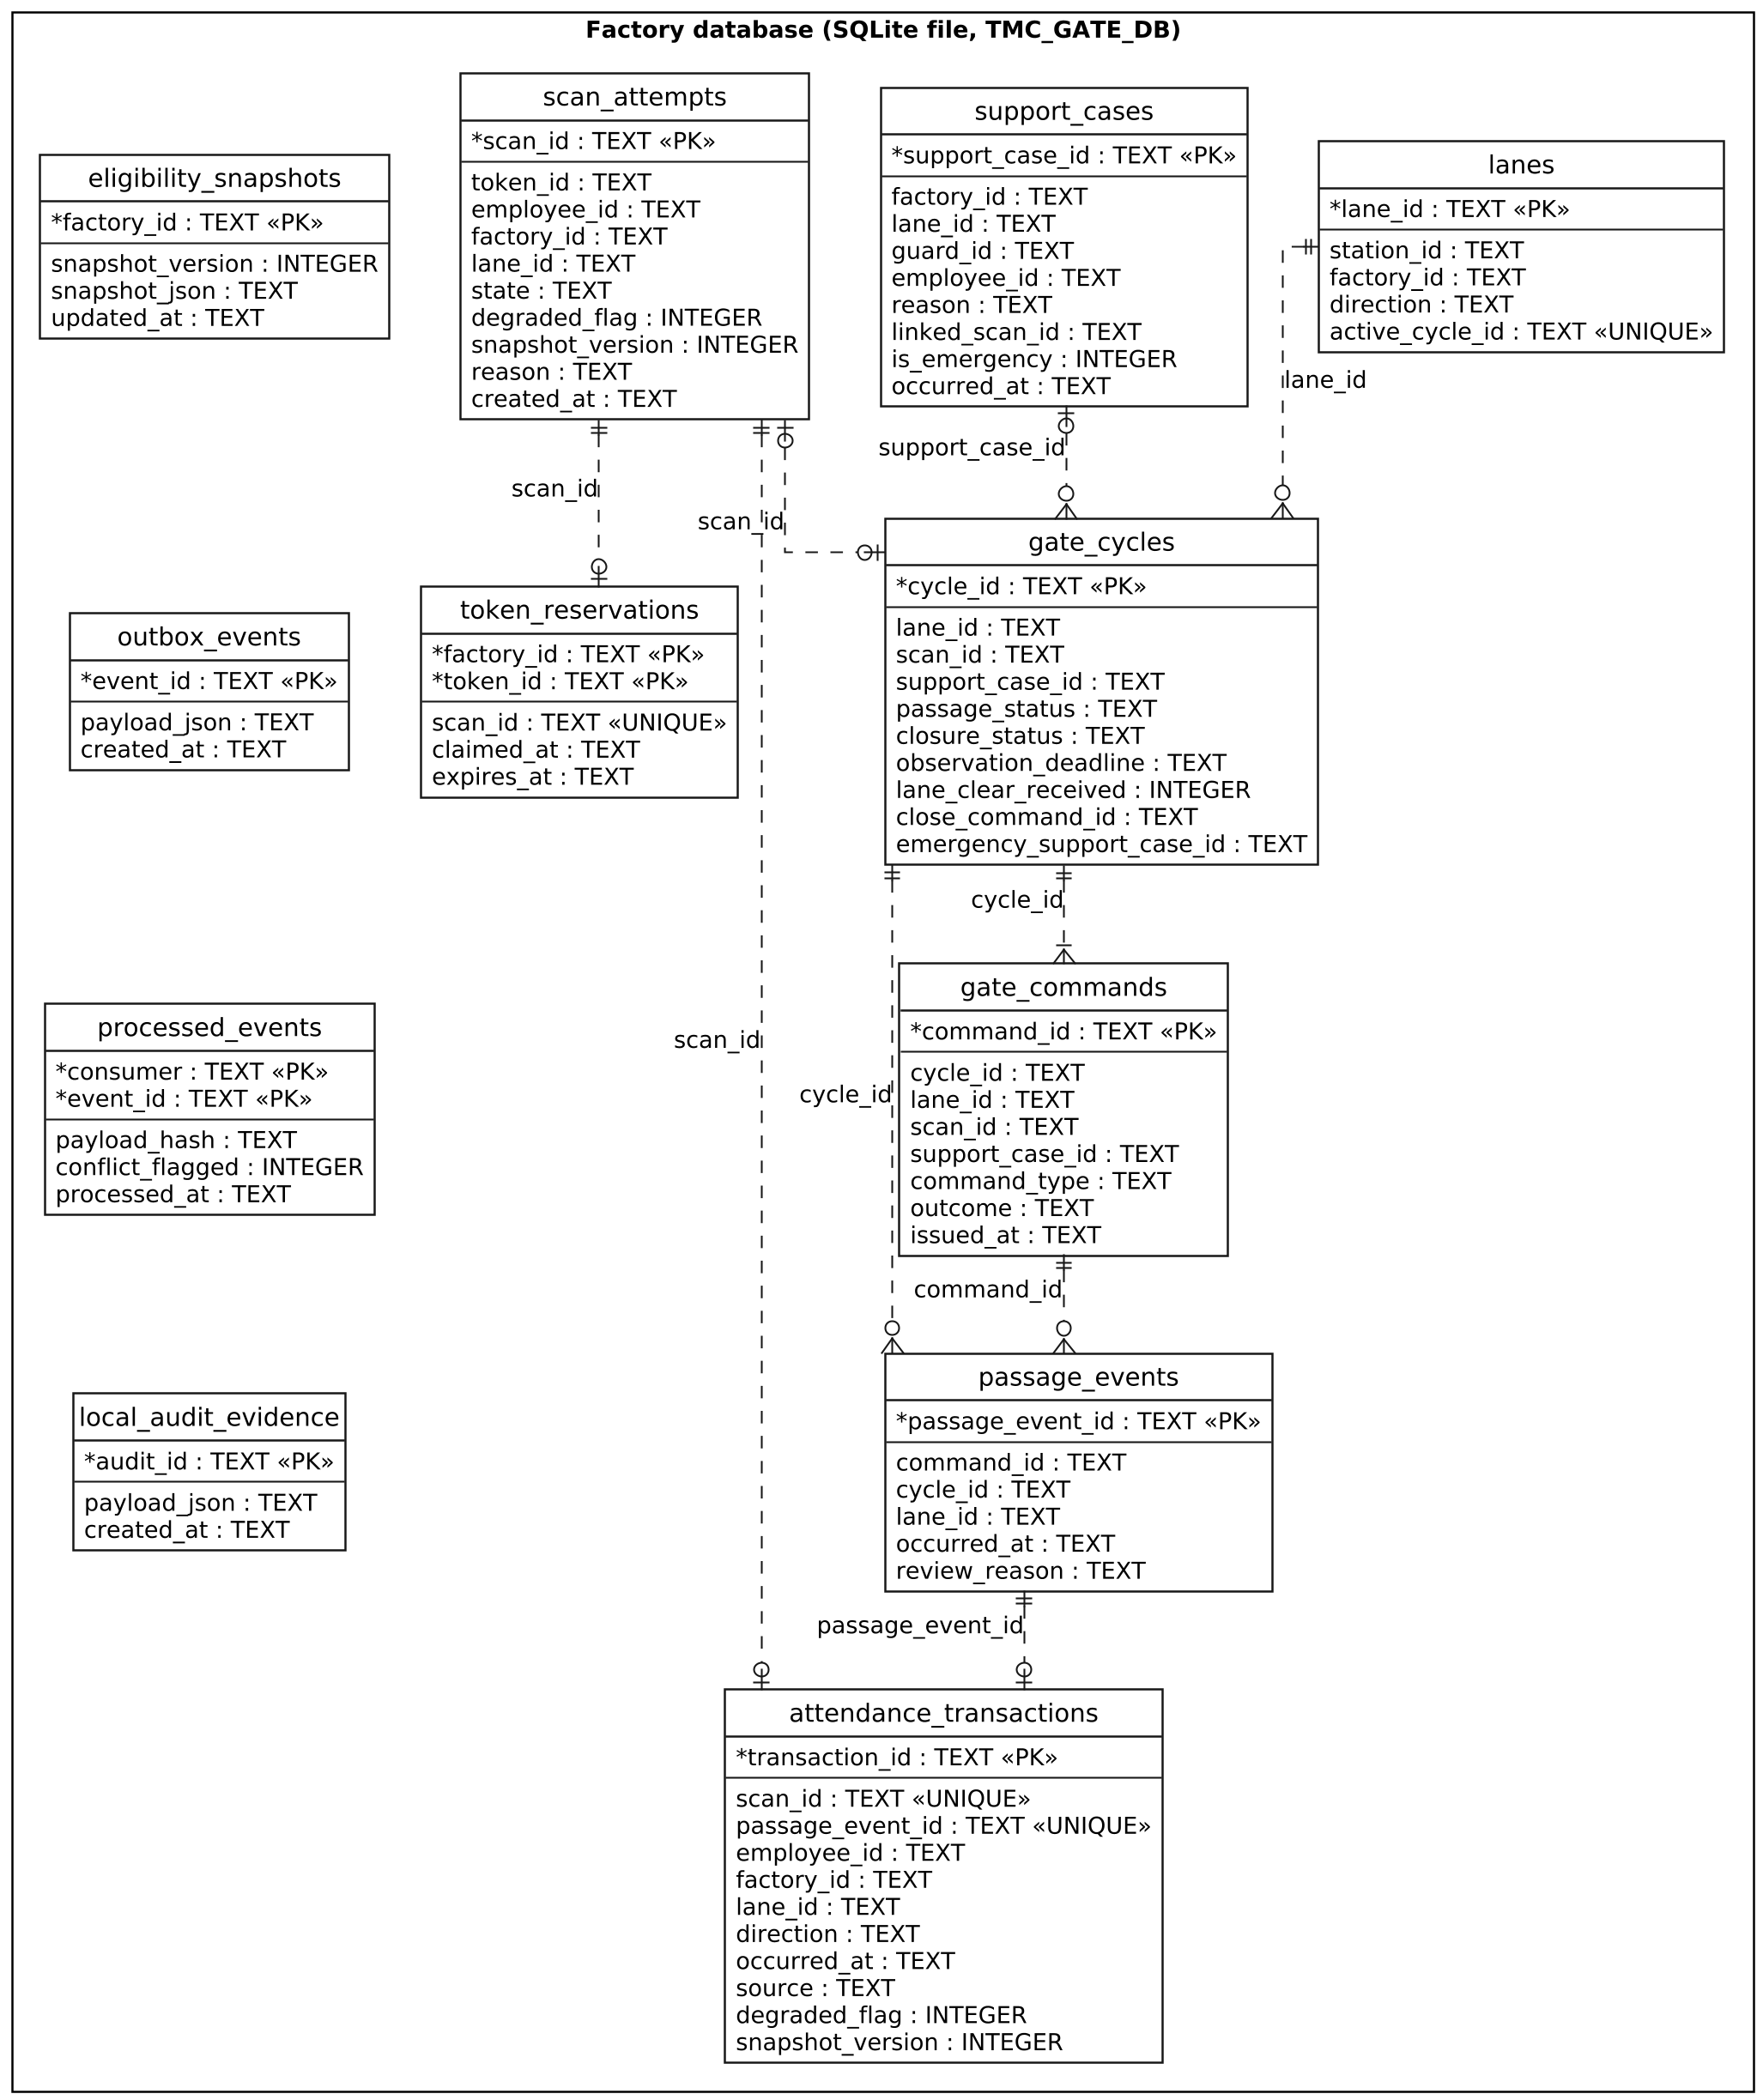
\includegraphics[width=\linewidth,height=430pt,keepaspectratio]{diagram/data/figure-9-2-data-view.png}}{\fbox{\parbox{300pt}{\centering\vspace{20pt}Figure being redrawn\vspace{20pt}}}}

\vspace{6pt}
\textbf{Figure 9.2. Data View of the Factory Database in the Prototype}
\phantomsection\addcontentsline{lof}{figure}{\protect\numberline{9.2}Data View of the Factory Database in the Prototype}
\end{minipage}

\vspace{10pt}

The schema has no foreign key constraints, so the dashed lines in Figure 9.2 are references kept by the code, not by SQLite. The rules that matter for duplicates are enforced by keys instead:

\begin{itemize}[leftmargin=36pt, itemsep=2pt, topsep=4pt, parsep=2pt]
  \item the primary key (factory\_id, token\_id) of \code{token_reservations} makes the claim of a QR token single-use, even for two connections at the same time;
  \item \code{lanes.active_cycle_id} holds at most one active cycle for each lane;
  \item \code{attendance_transactions} has unique scan\_id and passage\_event\_id, so one scan and one PASSAGE give at most one attendance record;
  \item the primary key of \code{passage_events} and of \code{processed_events} (consumer, event\_id) turn a repeated signal or event into a duplicate instead of a second row.
\end{itemize}

A file database runs in write-ahead logging mode, and the unit of work wraps each step of a flow in one transaction.

\Needspace{9\baselineskip}
\subsubsection*{9.3.4. HTTP Endpoints}

\phantomsection
\addcontentsline{toc}{subsubsection}{9.3.4. HTTP Endpoints}

Figure 9.3 is a screenshot of the Swagger page of the running prototype. The endpoints are grouped by who calls them. The kiosk uses the two scan endpoints, which only reach IScanSubmission. The two signal endpoints take PASSAGE and LANE\_CLEAR and reach IPassageEvents; in the prototype they are called by the demo script, Swagger UI, or the tests in place of a real controller. Guards use the three intervention endpoints and must send an \texttt{X-Guard-Session} header, because the guard is taken from the session and not from the request body. The four demo endpoints issue QR codes, change the age of the access data, choose how the simulated controller answers, and list the stored attendance. They are only mounted when \code{demo_mode} is on.

\noindent\begin{minipage}{\linewidth}
\centering
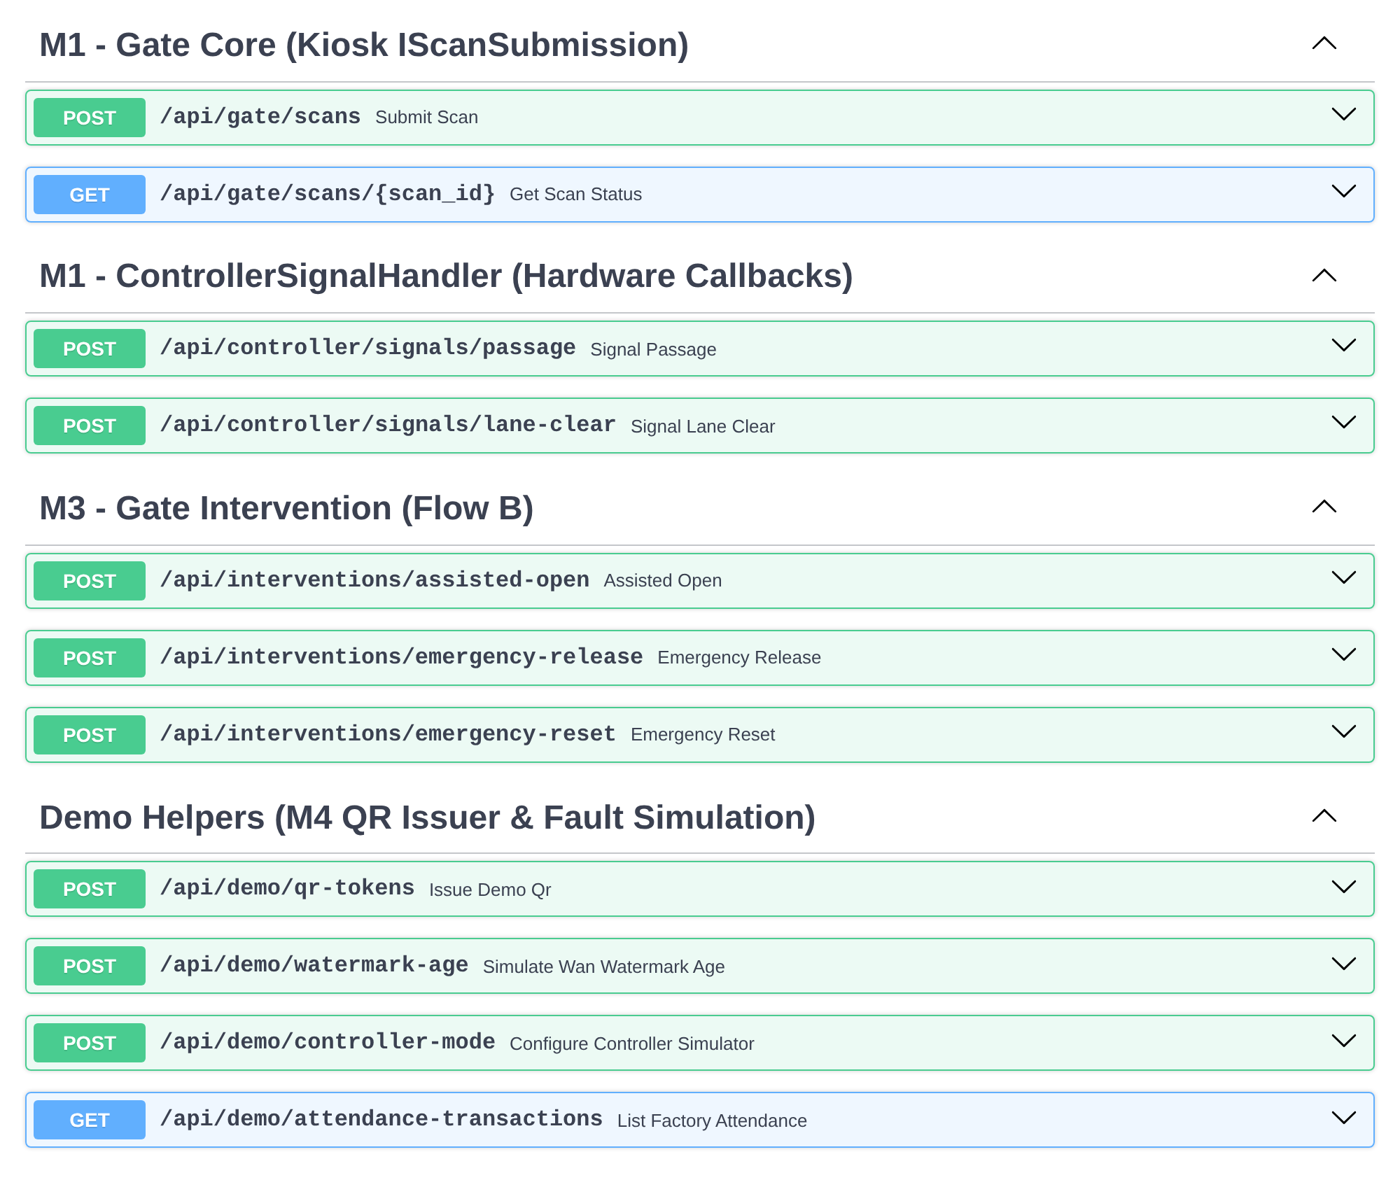
\includegraphics[width=0.82\linewidth]{figure/figure-9-3-swagger-endpoints.png}

\vspace{6pt}
\textbf{Figure 9.3. Endpoints of the Prototype in Swagger UI}
\phantomsection\addcontentsline{lof}{figure}{\protect\numberline{9.3}Endpoints of the Prototype in Swagger UI}
\end{minipage}

\vspace{10pt}

Table 9.5 lists the same endpoints with what each router is given in \code{app.py}. The kiosk and signal routes are typed with a port, so the dependency they declare is narrow. This is not an access control by itself: in Python, \code{app.py} still passes the whole GateCoreFacade object to the kiosk router. What keeps a kiosk from starting an intervention is that no kiosk endpoint calls such an operation, and that the guard endpoints check the guard session on the server. The guard routes get GateInterventionFacade and, for that session check, IGuardIdentityApi. The demo routes are wired directly to demo helpers, which is acceptable only because they are not mounted outside demo mode.

\noindent\begin{minipage}{\linewidth}
\centering
\begin{tabular}{|>{\raggedright\arraybackslash}p{167pt}|>{\raggedright\arraybackslash}p{56pt}|>{\raggedright\arraybackslash}p{88pt}|>{\raggedright\arraybackslash}p{84pt}|}
\hline
\multicolumn{1}{|>{\columncolor{tableheader}\centering\arraybackslash}p{167pt}|}{\textbf{Method and path}} & \multicolumn{1}{>{\columncolor{tableheader}\centering\arraybackslash}p{56pt}|}{\textbf{Caller}} & \multicolumn{1}{>{\columncolor{tableheader}\centering\arraybackslash}p{88pt}|}{\textbf{Router is given}} & \multicolumn{1}{>{\columncolor{tableheader}\centering\arraybackslash}p{84pt}|}{\textbf{Result}} \\
\hline
\code{POST /api/gate/scans} & Kiosk & IScanSubmission & Scan state, reason, commandId (A1--A7) \\
\hline
\code{GET /api/gate/scans/{scanId}} & Kiosk & IScanSubmission & Stored state after a lost response; 404 if unknown \\
\hline
\code{POST /api/controller/signals/passage} & Controller (played) & IPassageEvents & PASSAGE handled (A8) \\
\hline
\code{POST /api/controller/signals/lane-clear} & Controller (played) & IPassageEvents & LANE\_CLEAR handled, closeGate (A9) \\
\hline
\code{POST /api/interventions/assisted-open} & Guard & GateIntervention\-Facade & Support case and assisted openGate; 401 without a session \\
\hline
\code{POST /api/interventions/emergency-release} & Guard & GateIntervention\-Facade & EMERGENCY\_\allowbreak HOLD on the lane \\
\hline
\code{POST /api/interventions/emergency-reset} & Guard & GateIntervention\-Facade & Reset of the emergency that holds the lane \\
\hline
\code{POST /api/demo/qr-tokens} & Demo only & QR issuer helper & Signed 60-second token \\
\hline
\code{POST /api/demo/watermark-age} & Demo only & Snapshot storage & Operating mode after ageing the watermark \\
\hline
\code{POST /api/demo/controller-mode} & Demo only & ControllerApi\-Client & How the next commands and queries are answered \\
\hline
\code{GET /api/demo/attendance-transactions} & Demo only & Attendance storage & Stored attendance records \\
\hline
\end{tabular}

\vspace{6pt}
\textbf{Table 9.5. HTTP Endpoints of the Prototype}
\end{minipage}

\vspace{10pt}
\phantomsection\addcontentsline{lot}{table}{\protect\numberline{9.5}HTTP Endpoints of the Prototype}

\Needspace{9\baselineskip}
\subsection*{9.4. SOLID in the Code}

\phantomsection
\addcontentsline{toc}{subsection}{9.4. SOLID in the Code}

Section 7.1 explains how SOLID shaped the modules on paper. Here we look at where each principle shows up in the code and, where one exists, which test checks it.

The single responsibility principle is about actors: a module should answer to one group of people who ask for the same kind of change. ``One reason to change'' says the same thing, as long as the reason is traced back to who asks for it. In our code, the gate rules are asked for by the people who run the factory gates and security, while shift and payroll rules come from HR. Because of I-06, a change in the shift or attendance rules of HR does not reach the gate decision: AccessDecision (\code{application/access_decision.py}) only checks the token against the snapshot and returns a DecisionResult, and it has no shift input and no turnstile port. The rules about how fresh the access data must be live in EligibilitySnapshot (\code{domain/snapshot.py}), and InterventionService only checks what a guard is allowed to do and leaves the gate commands to Gate Core.

GateTransactionProcessor is the largest class, and its size alone does not show that SRP holds or fails. Its responsibility is to coordinate the life cycle of one gate transaction: accept the scan, reserve the lane, open, handle PASSAGE and LANE\_CLEAR, close, and handle the emergency commands on the same lane. The eligibility check, the storage, and the controller protocol have been moved out to AccessDecision, the repositories, and the adapters, so a change in one of them does not edit the processor. GateCoreFacade is a thin entry point that turns the inbound ports into processor calls; its name is not evidence of SRP either. Because of the split, \code{test_pkg1_snapshot.py} can test the snapshot rules alone, and \code{test_pkg2_access_decision.py} can call AccessDecision.evaluate twice on the same data and check that it gives the same answer without changing anything.

For the open/closed principle, the place that changes is the controller. The ports in \code{ports/turnstile.py} belong to Gate Core, and the adapters depend on them, not the other way round. A new turnstile model would be a new class in \code{adapters/} that implements ITurnstileControl, and \code{api/app.py} decides which adapter is passed in. This is close to the Strategy idea from the lecture: the processor keeps its rules and only the object behind the port is swapped. \code{test_pkg5_adapter_with_processor.py} runs the same GateTransactionProcessor with both adapter classes we have, and the processor did not need any change for the second one.

The Liskov substitution principle matters most for the meaning of a controller result. The port file \code{ports/turnstile.py} fixes the set of results that each command may return. A receipt or a timeout must come back as UNDETERMINED, not as OPEN\_CONFIRMED or CONTROLLER\_ERROR. One contract test file, \code{test_pkg5_turnstile_contract.py}, runs the same checks against SimulatedTurnstileAdapter and FaultyTurnstileAdapter, and both pass. We also wrote a third adapter that reports a receipt as OPEN\_CONFIRMED. It fails the same contract, and this test is marked as an expected failure on purpose.

Interface segregation is judged from the consumer's side. It shows in how GateCoreApi is split into IScanSubmission, IInterventionRequest, and IFactoryUpdates (\code{ports/inbound.py}). The kiosk router only receives IScanSubmission, InterventionService only receives IInterventionRequest, and the controller routes only receive IPassageEvents. On the other side, the processor depends on IOpenGate, ICloseGate, and IEmergencyGate one by one, even though one adapter class implements all three as ITurnstileControl. \code{test_interface_segregation_principle_contracts} checks that the kiosk interface has no intervention or sync operation and that IPassageEvents has only onPassage and onLaneClear. The split is not complete everywhere: IScanRepository still has 14 operations, all used by the processor, while GateCoreFacade only uses get\_scan and save\_scan. Section 8.2 discusses this limitation.

Dependency inversion is what made the group work possible. GateTransactionProcessor receives all its ports and its IUnitOfWork through the constructor, and the application layer does not import \texttt{sqlite3}, \texttt{fastapi}, \code{adapters/}, or \code{api/}. \code{api/app.py} is the composition root: it creates the main dependencies (the SQLite repositories and unit of work, the turnstile adapter, the processor, the facades, and the timeout worker) and connects them. In \code{test_architecture_solid.py}, three import tests check the domain, ports, and application layers one by one, and a fourth test checks the ISP splits. These tests check the direction of dependencies and the shape of the ports; they do not prove all five principles, and SRP and OCP in particular are design judgements supported by the examples above. We wrote and merged the ports before anything else, so six people could work in parallel against fakes. Packages 1, 3, and 6 were finished and tested before the SQLite repositories or the turnstile adapter existed.

Only one port was added after that point. While checking the code before submission we found that a cycle with no PASSAGE could stay OPENED, because nothing triggered the 15-second timeout once LANE\_CLEAR had already released the lane. The processor needed a way to find such cycles by their own state, so we added the small read port IPassageWindowQuery (\code{list_cycles_awaiting_passage}, \code{get_cycle_by_scan}) instead of putting two more methods on IScanRepository. SqliteScanRepository implements it, and PassageTimeoutWorker uses it through the processor (Section 9.5, step A8).

\Needspace{9\baselineskip}
\subsection*{9.5. Following One Scan Through the Code}

\phantomsection
\addcontentsline{toc}{subsection}{9.5. Following One Scan Through the Code}

The tables above show what exists, but not in which order things happen. In this section we follow one QR scan from the kiosk request to the closed gate. Each step carries the label of the matching step in the design sequence of Figure 4.16 and Section 4.2.2, so the two descriptions can be read side by side. The classes are the ones in Figures 4.18 and 4.19, and Figure 9.4 draws the same steps as two sequence diagrams with the names used in the code. Part (a) is the kiosk request, A1 to A7. Part (b) shows A8 and A9, which arrive as their own HTTP requests. Both parts show one successful run as an example. The order in which they are drawn is not an order the code guarantees: the PASSAGE request can be handled before the kiosk has received its A7 response, and LANE\_CLEAR does not wait for PASSAGE.

\noindent\begin{minipage}{\linewidth}
\centering
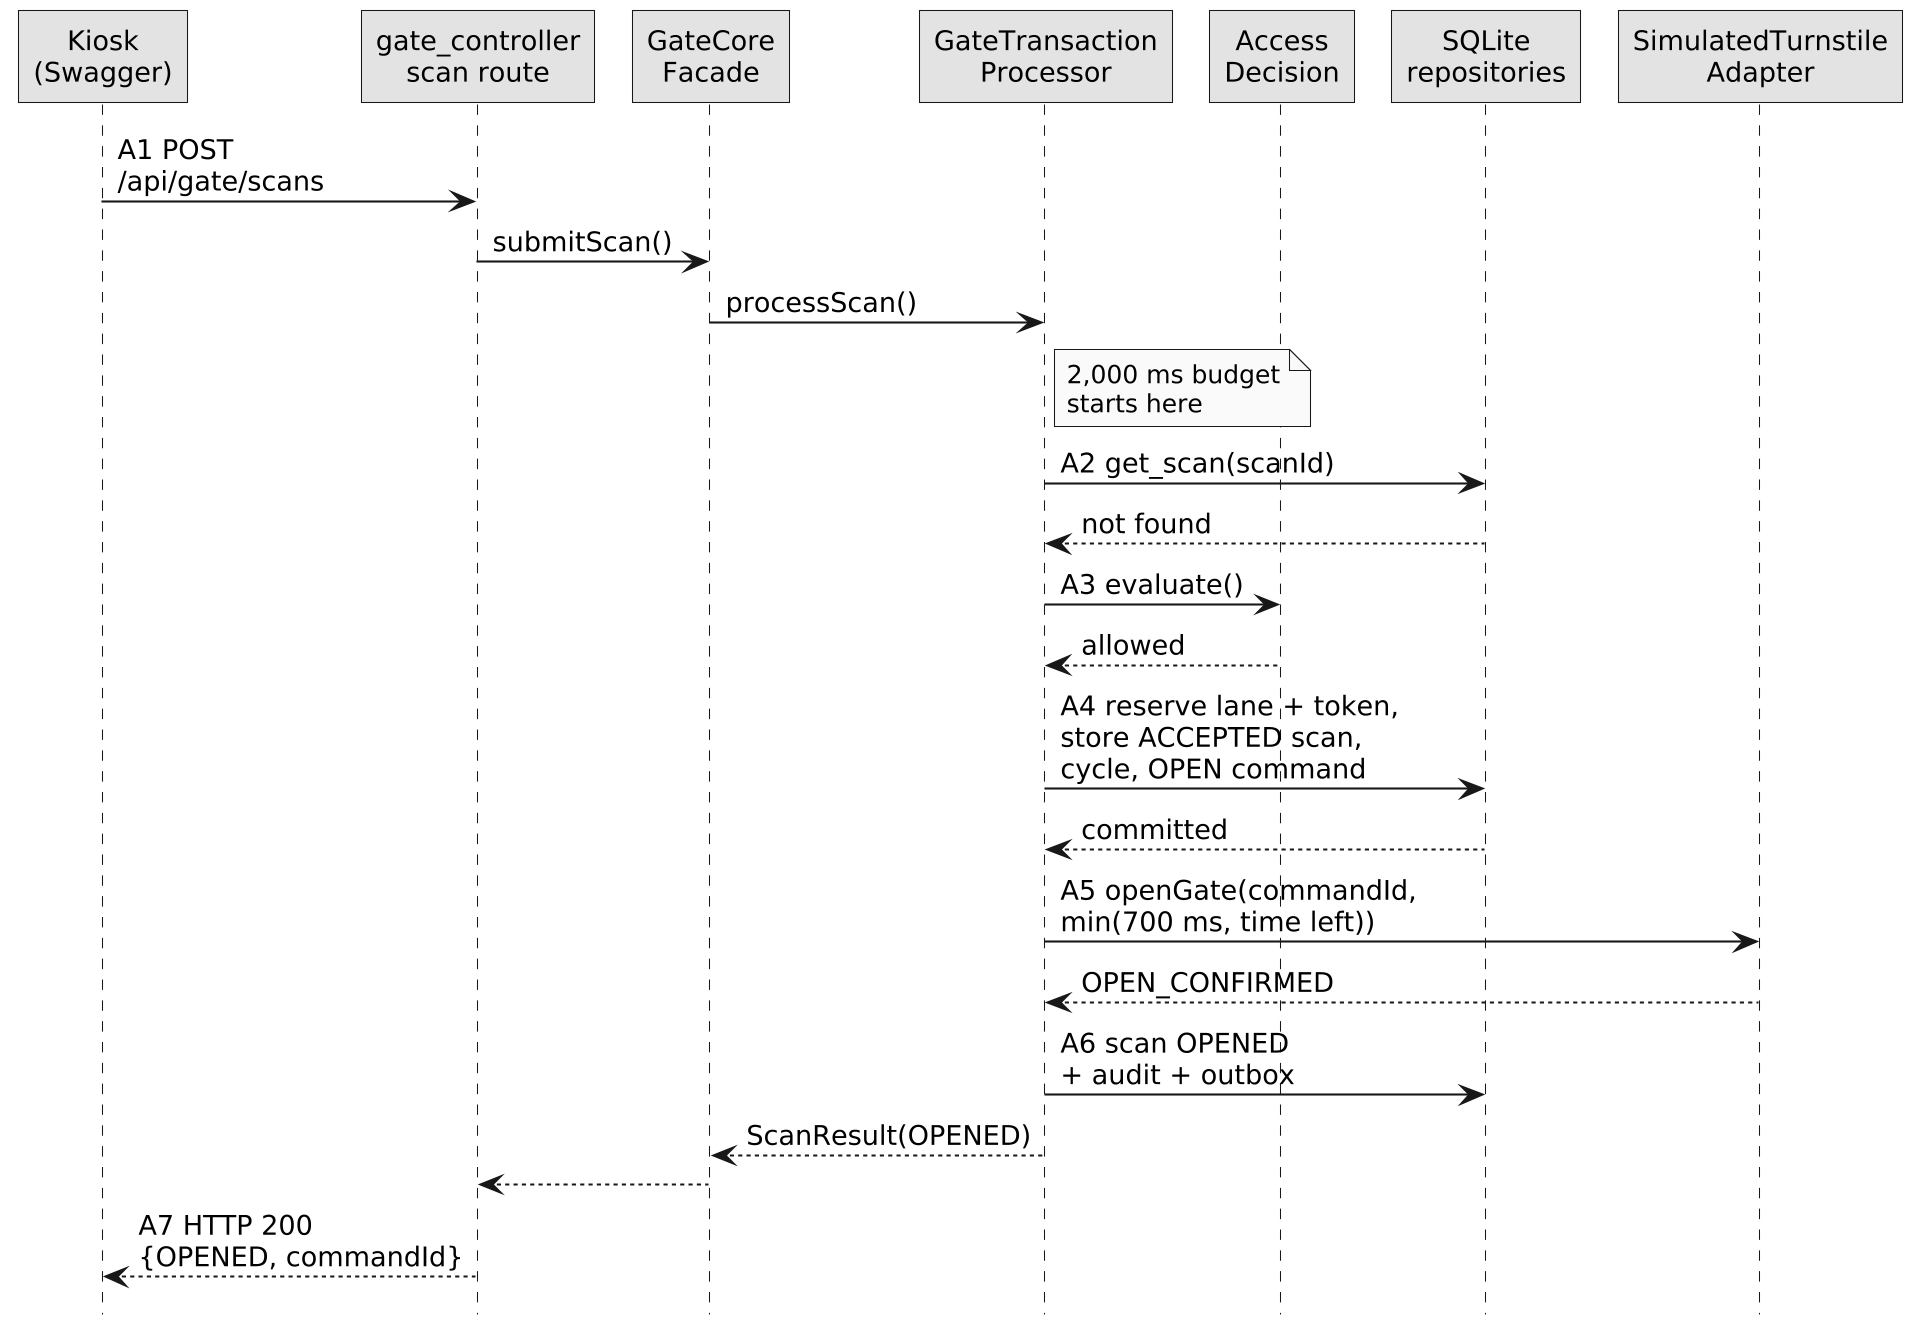
\includegraphics[width=0.94\linewidth]{diagram/implementation/figure-9-4a-scan-request.png}

\vspace{2pt}
{\small (a) Kiosk request, A1--A7}
\end{minipage}

\vspace{8pt}
\noindent\begin{minipage}{\linewidth}
\centering
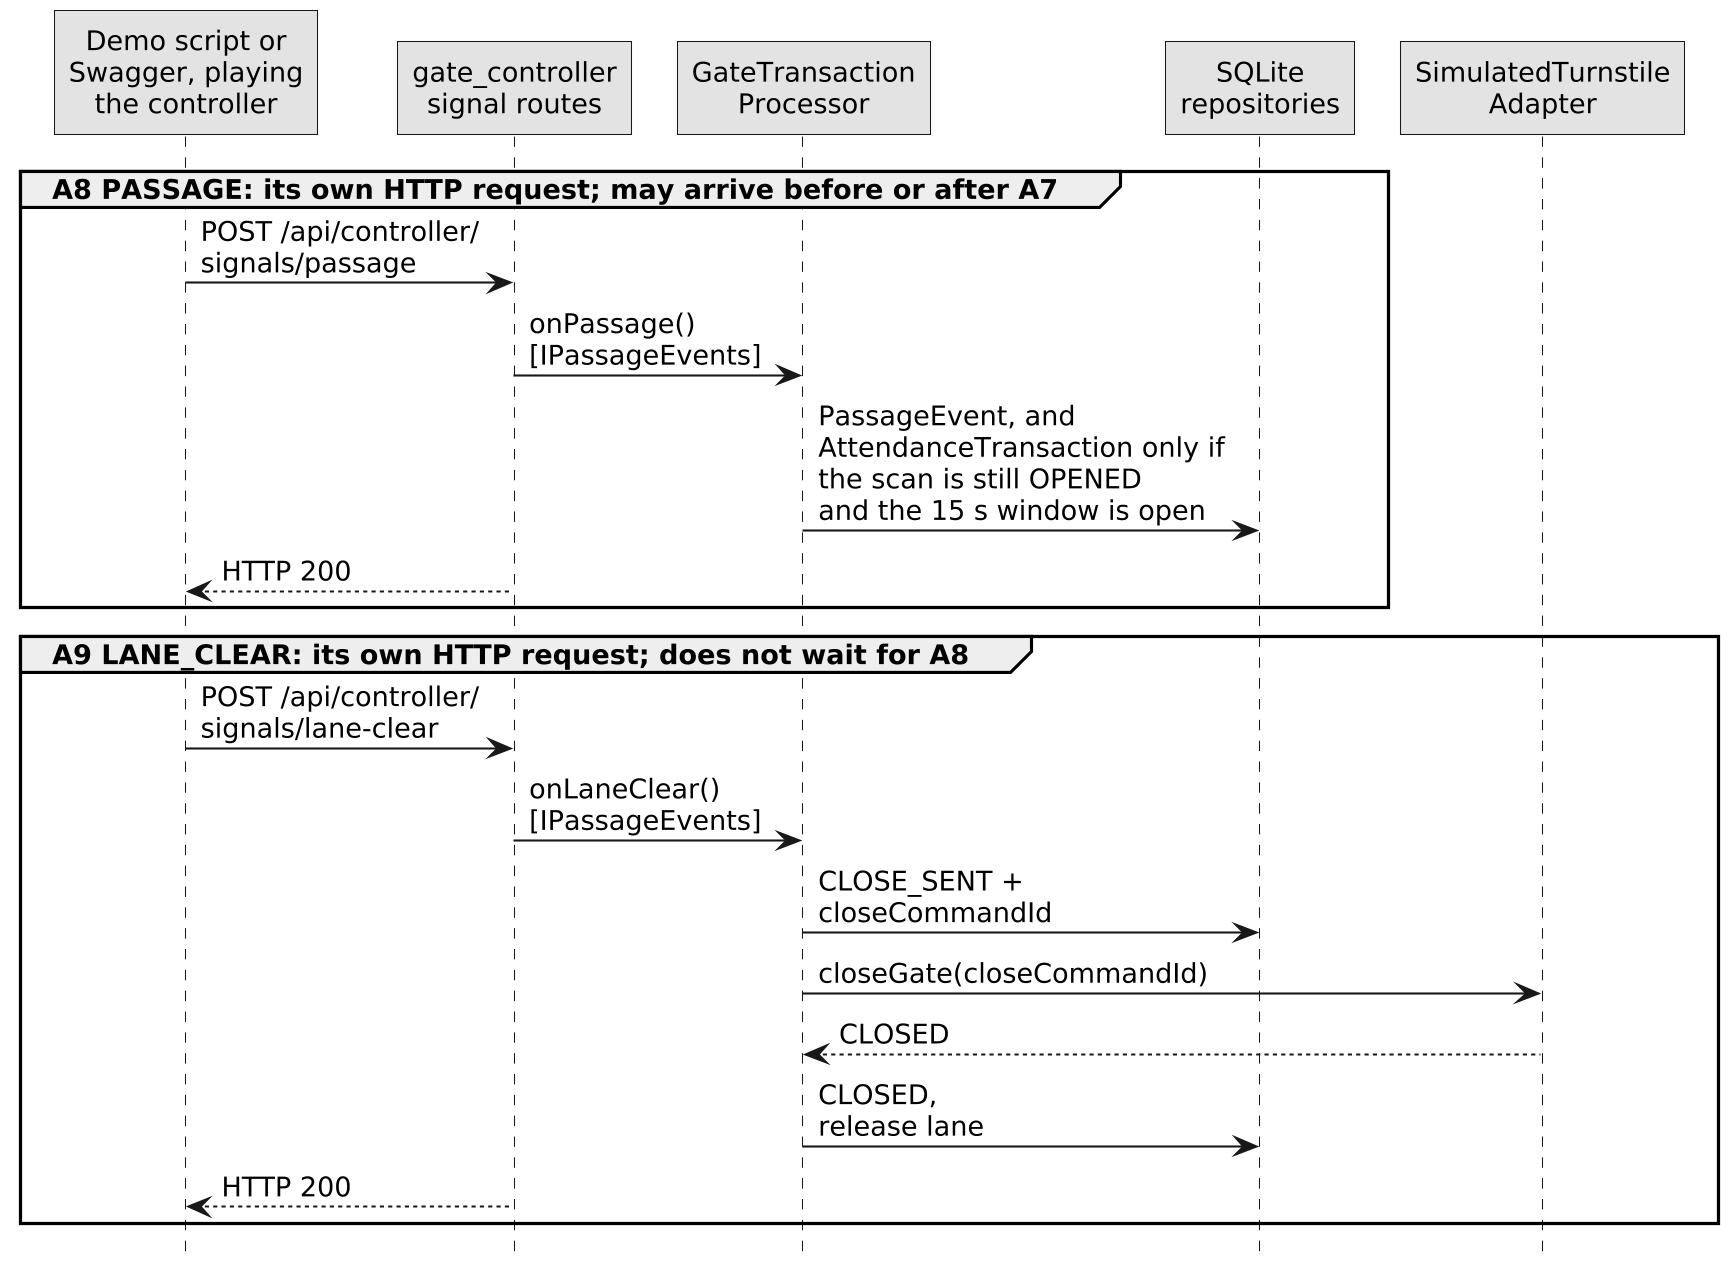
\includegraphics[width=0.86\linewidth]{diagram/implementation/figure-9-4b-controller-signals.png}

\vspace{2pt}
{\small (b) Controller signals, A8 and A9: separate requests, in any order relative to (a) and to each other}

\vspace{6pt}
\textbf{Figure 9.4. Flow A as Implemented: One Scan from the Kiosk Request to the Closed Gate}
\phantomsection\addcontentsline{lof}{figure}{\protect\numberline{9.4}Flow A as Implemented}
\end{minipage}

\vspace{10pt}

\begin{itemize}[leftmargin=36pt, labelwidth=22pt, labelsep=8pt, align=left, itemsep=3pt, topsep=4pt, parsep=2pt]
  \item[\textbf{A1}] The kiosk sends \code{POST /api/gate/scans} with a scanId, the QR text, and the laneId. The route only holds an IScanSubmission, so it calls GateCoreFacade.submitScan, which hands the scan to GateTransactionProcessor.processScan. From here the processor counts down a processing budget, and every later step only gets the time that is left. The HTTP route does not pass a kiosk deadline, so this budget is a full 2,000 ms that starts when processScan begins (Section 9.8).
  \item[\textbf{A2}] The processor first looks the scanId up in storage. If the kiosk is retrying a request whose answer was lost, the stored result is returned unchanged and nothing else runs.
  \item[\textbf{A3}] AccessDecision.evaluate reads the current EligibilitySnapshot and checks the operating mode first. If the access data is too old or the clock error is too large, the answer is CANNOT\_PROCESS before the QR code is even read. Otherwise it verifies the Ed25519 signature, the 60-second expiry, and the factory of the token, and then asks the snapshot whether this employee may use this lane. A scan that fails is stored as REJECTED or CANNOT\_PROCESS with an audit record, and the kiosk gets the reason.
  \item[\textbf{A4}] For an allowed scan the processor prepares four records: the ACCEPTED ScanAttempt, a TokenReservation for the tokenId, a new GateCycle for the lane, and the OPEN GateCommand. SqliteScanRepository writes all four in one transaction. If the lane already has an active cycle, nothing is written and the answer is LANE\_BUSY. If the tokenId has been claimed before, for example by a copy of the QR code on another lane, the scan is stored as REJECTED with the reason QR\_TOKEN\_REPLAY\_DETECTED.
  \item[\textbf{A5}] Only after this commit does the processor call openGate, with a timeout of min(700 ms, time left). If no time is left at this point, the command is not sent: the scan ends as CANNOT\_PROCESS and the lane is released, but the token stays claimed.
  \item[\textbf{A6}] The controller result decides the next state. With OPEN\_CONFIRMED the scan becomes OPENED and the 15-second passage window starts; the outbox event and the audit record go into the same transaction. With CONTROLLER\_ERROR the lane is released. An UNDETERMINED result is stored first, and the controller is asked once through IControllerStatusQuery where the adapter supports it. If there is no status query, or the answer is still unclear, the scan becomes PENDING\_RECONCILIATION.
  \item[\textbf{A7}] processScan returns this state to the route, and the kiosk receives it in the HTTP response. This is where the server-side part of the scan ends. NFR-01 itself is measured until the kiosk displays the result (Section 1.7), and the prototype does not measure that. Returning the opening result does not create attendance. Attendance is recorded separately when a valid PASSAGE is processed, independently of when the kiosk receives its response.
  \item[\textbf{A8}] Attendance comes from the passage, not from the opening. When the employee walks through, the controller calls \code{POST /api/controller/signals/passage}. This request reaches onPassage on the processor through IPassageEvents, and it is handled on its own, separately from the kiosk request. In one transaction the processor stores the PassageEvent and, if the scan is still OPENED and the window has not ended, the AttendanceTransaction. A passage that comes too late is still stored, but with the review reason LATE\_PASSAGE and without attendance. If no PASSAGE arrives at all, PassageTimeoutWorker, which wakes up every 0.25 seconds, makes the processor mark the cycle as NO\_PASSAGE and the scan as PENDING\_RECONCILIATION once the 15 seconds are over. The worker does not close the gate.
  \item[\textbf{A9}] Closing waits for LANE\_CLEAR, whether or not a passage was recorded. The signal arrives at \code{/api/controller/signals/lane-clear}, and onLaneClear first stores CLOSE\_SENT and the closeCommandId. Only then does it call closeGate. The lane becomes free again when the result is CLOSED.
\end{itemize}

We also ran these steps by hand on a team member's Windows laptop, against a real \texttt{uvicorn} server in demo mode, with \code{TMC_GATE_DB} pointing to a SQLite file and the simulated controller. The server ran in one PowerShell window and the client in a second one, using the script \code{report/evidence/run_demo.py}. Figure 9.5 is a screenshot of the second window. The script first marks the access data as just confirmed, because the prototype has no Site Sync and the server only treats its data as fresh at start-up; without this step a run started more than 60 seconds after the server would come out DEGRADED. We took a signed QR code for employee EMP-001 from the demo endpoint and used it twice: S-1 on LANE-BD-01 was OPENED (a), and S-2 with the same code on LANE-BD-02 was REJECTED with QR\_TOKEN\_REPLAY\_DETECTED (b). We then played the controller and sent PASSAGE and LANE\_CLEAR twice each for the commandId of S-1 (c). The HTTP answers alone do not show that the repeats were ignored, so in (d) we opened the database file with a separate connection. It holds one attendance record, linked to S-1 and passage event PE-1, one passage event, and exactly one OPEN and one CLOSE command. Table 9.8 in Section 9.7 sums up what each part of the run shows.

\noindent\begin{minipage}{\linewidth}
\centering
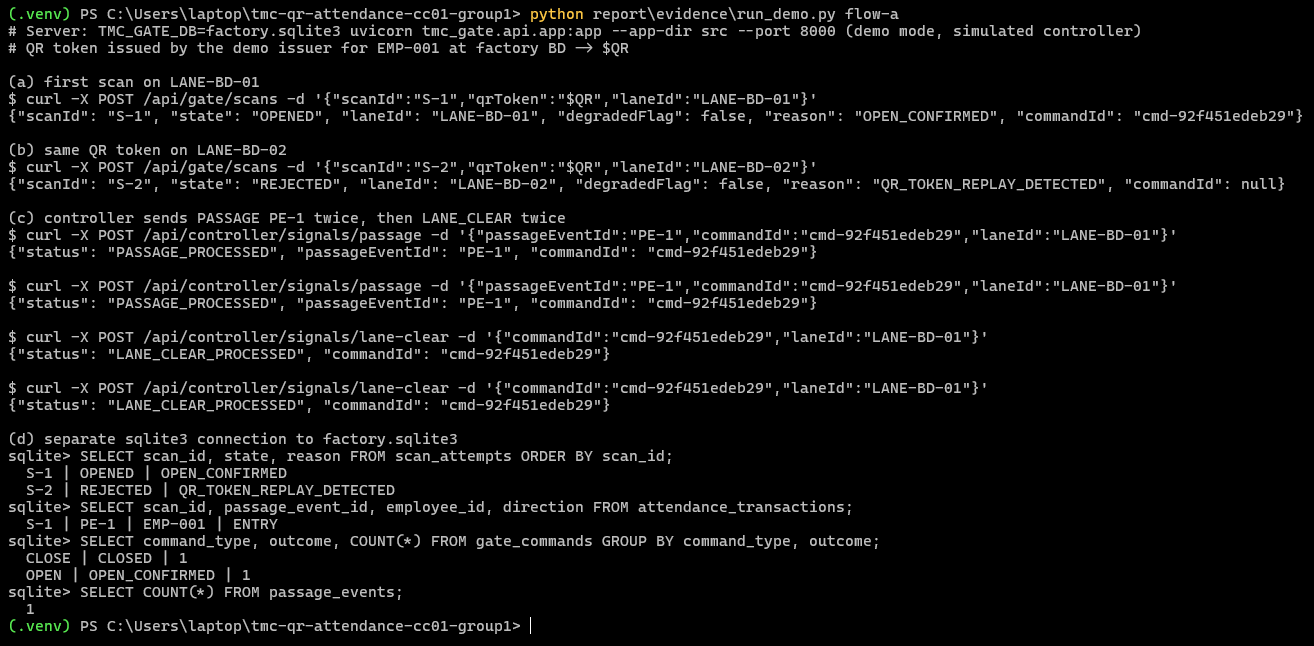
\includegraphics[width=\linewidth]{figure/figure-9-5-flow-a-run.png}

\vspace{6pt}
\textbf{Figure 9.5. Flow A on Uvicorn with a SQLite File: Repeated Signals Give One Attendance Record}
\phantomsection\addcontentsline{lof}{figure}{\protect\numberline{9.5}Flow A on Uvicorn with a SQLite File}
\end{minipage}

\vspace{10pt}

The run in Figure 9.5 only covers the normal path. We ran the same script twice more, each time with a fresh SQLite file, to show what happens when something is not normal. In Figure 9.6 we first aged the access data to 300 seconds: scan S-10 was still OPENED, but with the degraded flag, and the attendance record created from its passage carries the same flag (a). At 1800 seconds the next scan was refused with CANNOT\_PROCESS before any command (b). We then made the access data fresh again and set the simulated controller so that openGate times out and the status query cannot tell the result. Scan S-12 ended as PENDING\_RECONCILIATION, and a new scan on the same lane got LANE\_BUSY because the lane stays held (c). The database shows a single OPEN command for S-12 with the outcome UNDETERMINED (d).

\noindent\begin{minipage}{\linewidth}
\centering
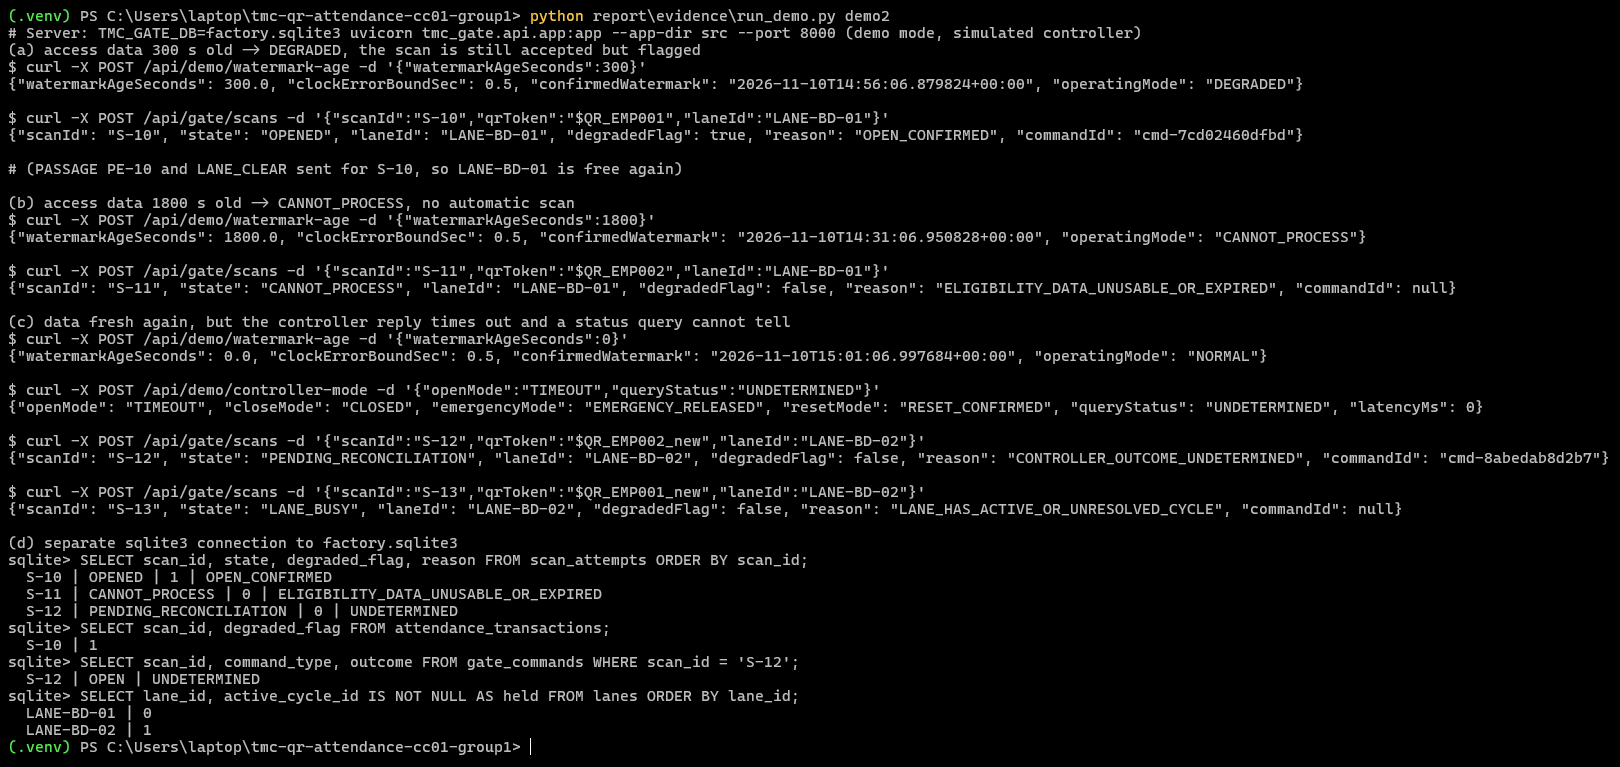
\includegraphics[width=\linewidth]{figure/figure-9-6-degraded-undetermined-run.png}

\vspace{6pt}
\textbf{Figure 9.6. Degraded Mode, CANNOT\_PROCESS, and an Uncertain Opening on Uvicorn}
\phantomsection\addcontentsline{lof}{figure}{\protect\numberline{9.6}Degraded Mode and an Uncertain Opening on Uvicorn}
\end{minipage}

\vspace{10pt}

Figure 9.7 runs the local part of Flow B. An assisted opening without a guard session gets HTTP 401 (a). With the session, the same request sent twice returns the same commandId both times (b). We then played the controller for this assisted opening and sent a PASSAGE right away, well inside the 15-second window, followed by LANE\_CLEAR (c). For a QR scan the same two signals created an attendance record in Figure 9.5. An emergency release puts LANE-BD-01 in EMERGENCY\_HOLD, and a QR scan on that lane gets LANE\_BUSY (d). After the reset and a LANE\_CLEAR the gate is closed and the next scan is OPENED again (e). In the database (f), case-001 has one stored OPEN command and one CLOSE command, the passage PE-30 is stored without a review reason, and there is still no attendance record. So a timely passage through an assisted opening did not create attendance by itself. The run does not show the later HR approval step, which is outside the prototype.

\noindent\begin{minipage}{\linewidth}
\centering
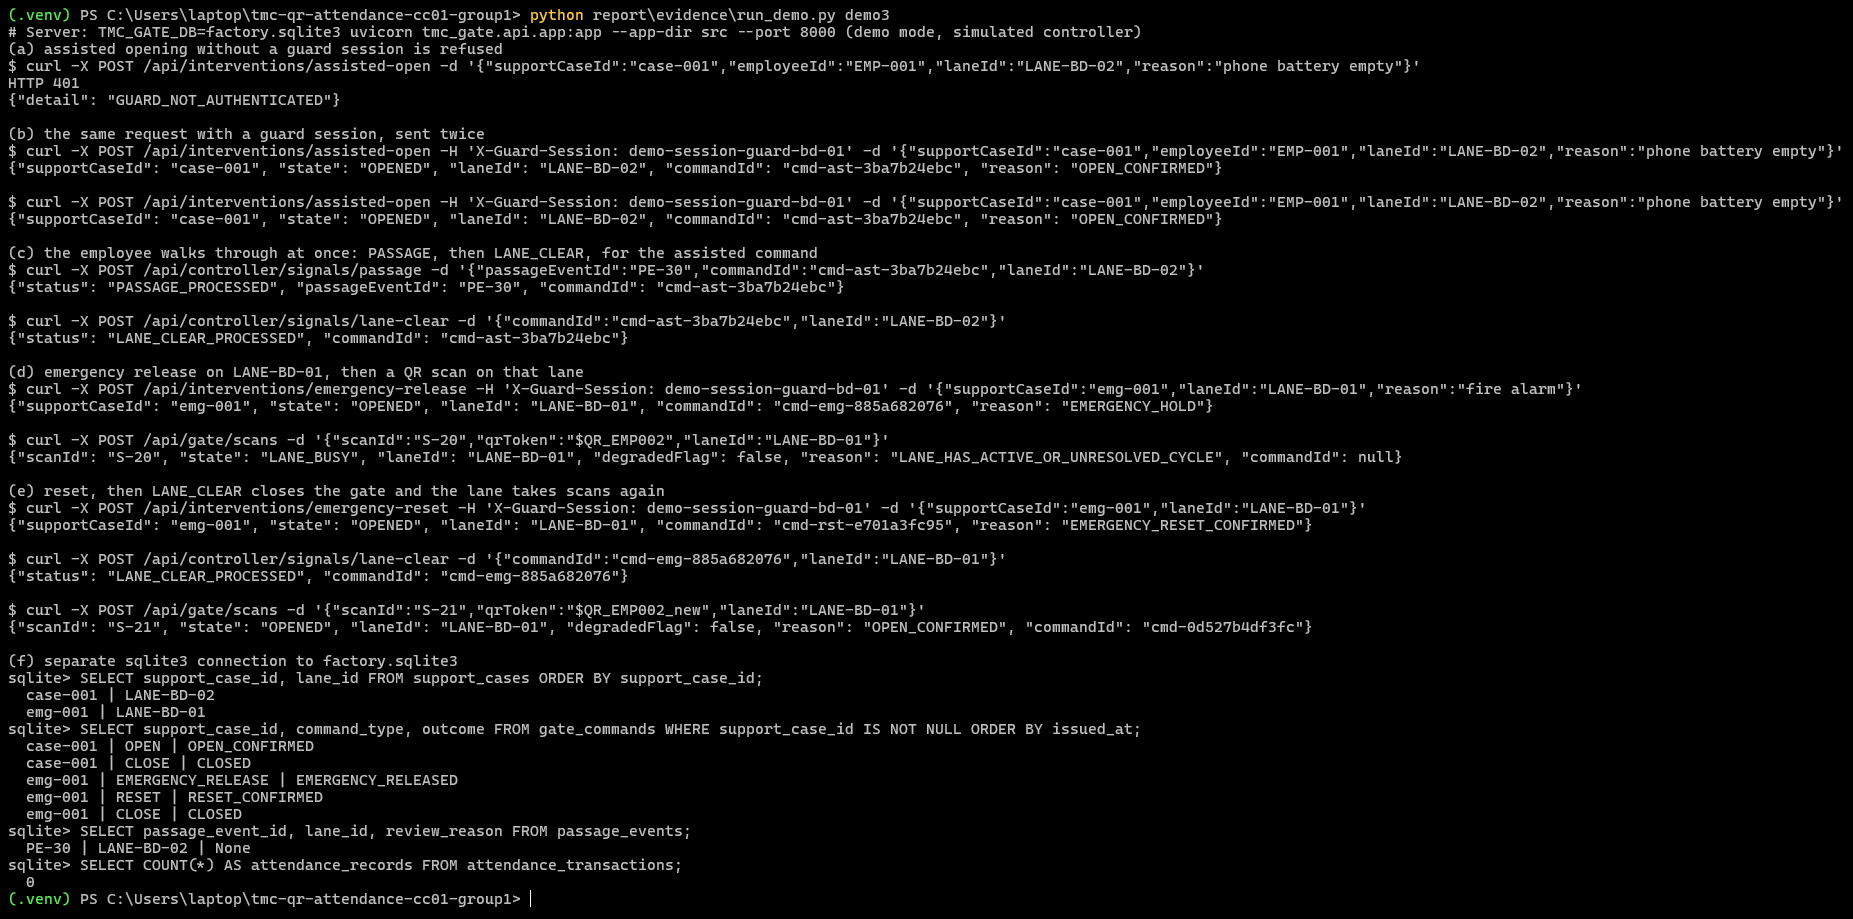
\includegraphics[width=\linewidth]{figure/figure-9-7-flow-b-run.png}

\vspace{6pt}
\textbf{Figure 9.7. Flow B on Uvicorn: Guard Session, Assisted Opening with a Passage, and Emergency Hold}
\phantomsection\addcontentsline{lof}{figure}{\protect\numberline{9.7}Flow B on Uvicorn}
\end{minipage}

\vspace{10pt}

\Needspace{9\baselineskip}
\subsection*{9.6. Design Rules Checked by Tests}

\phantomsection
\addcontentsline{toc}{subsection}{9.6. Design Rules Checked by Tests}

Before the numbers, Table 9.6 links the main gate rules of Chapters 4 to 7 to the tests that check them. Unless the table says otherwise, these tests use in-memory fakes for storage and for the controller, so they check the logic of Gate Core and Gate Intervention rather than the behavior of a real database.

\begin{longtable}{|>{\raggedright\arraybackslash}p{60.5pt}|>{\raggedright\arraybackslash}p{180.5pt}|>{\raggedright\arraybackslash}p{169.5pt}|}
\hline
\multicolumn{1}{|>{\columncolor{tableheader}\centering\arraybackslash}p{60.5pt}|}{\textbf{Source}} & \multicolumn{1}{>{\columncolor{tableheader}\centering\arraybackslash}p{180.5pt}|}{\textbf{Rule}} & \multicolumn{1}{>{\columncolor{tableheader}\centering\arraybackslash}p{169.5pt}|}{\textbf{Test file}} \\
\hline
\endhead
\multicolumn{3}{c}{\rule{0pt}{20pt}\normalsize\textbf{Table 9.6. Design Rules and Their Tests}} \\
\endlastfoot
Flow A, ADR-02 & ACCEPTED, the token claim, and the new GateCycle are stored before openGate; a busy lane returns LANE\_BUSY without claiming the token. & \code{test_pkg3_processor.py}, \code{test_pkg4_sqlite_repos.py}, \code{test_e2e_sqlite_flows.py} \\
\hline
Table 5.5 & openGate gets min(700 ms, time left of the 2-second budget); if no time is left, the scan ends as CANNOT\_PROCESS, the lane is released, and the token stays claimed. & \code{test_pkg3_rules.py}, \code{test_pkg3_pr2_regressions.py} \\
\hline
I-03, Section 7.1.3 & An UNDETERMINED opening is stored, queried once where the port exists, and then moved to PENDING\_RECONCILIATION. The same scan never gets a second open command. & \code{test_pkg3_rules.py}, \code{test_pkg3_pr2_regressions.py}, \code{test_pkg5_adapter_with_processor.py} \\
\hline
I-07, ADR-02 & Attendance is created only after a stored PASSAGE while the scan is still OPENED within 15 seconds; a repeated passageEventId is ignored, a second passage is kept without attendance, and a late passage is stored as LATE\_PASSAGE for review. & \code{test_pkg3_rules.py}, \code{test_pkg3_pr2_regressions.py} \\
\hline
I-05, Table 4.23b & closeGate is sent once after LANE\_CLEAR; the 15-second timer never closes the gate; an old close result cannot release a lane that a new scan holds. & \code{test_pkg3_rules.py}, \code{test_pkg3_pr2_followup.py} \\
\hline
I-10, Section 5.7.2 & NORMAL up to 60 s, DEGRADED below 30 min, CANNOT\_PROCESS from 30 min, or when the clock error bound is unknown or at least 2 s, or the data is not continuous. & \code{test_pkg1_snapshot.py} \\
\hline
ADR-11 & Ed25519 signature, 60-second expiry, factory binding, and single-use claim of tokenId. & \code{test_pkg2_*.py}; two connections claiming one token: \code{test_pkg4_sqlite_repos.py}; copied QR on another lane: \code{test_e2e_sqlite_flows.py} \\
\hline
Flow B, ADR-07 & Assisted opening needs an authorized guard, uses its own 3-second timeout, and creates no attendance; one openGate per supportCaseId, also for two requests at the same time; guardId comes from the session, not the request body. & \code{test_pkg6_intervention.py}, \code{test_pkg6_pr8_*.py}, \code{test_pkg3_rules.py}, \code{test_final_code_edges_regressions.py} \\*
\hline\noalign{\nobreak}
Flow B & Emergency release puts the lane in EMERGENCY\_HOLD and blocks new scans; only RESET\_CONFIRMED for the emergency that holds the lane now ends the hold, so a late reset result for an older emergency returns EMERGENCY\_SUPERSEDED. The RESET command is stored before it is sent. An uncertain result reuses and queries that command; only controller-confirmed non-execution (CONTROLLER\_ERROR) permits a new RESET command. & \code{test_pkg6_intervention.py}, \code{test_pkg3_pr2_regressions.py}, \code{test_final_code_edges_regressions.py} \\
\hline
Flow B & An emergency wins over an open result that arrives after it: a late OPEN\_CONFIRMED creates no attendance, and a late CONTROLLER\_ERROR does not release the held lane. & \code{test_submission_audit_regressions.py}, \code{test_pr15_followup_regressions.py} \\
\hline
Table 4.23b & With no PASSAGE within 15 seconds, the worker moves the cycle to NO\_PASSAGE and the scan to PENDING\_RECONCILIATION, also after LANE\_CLEAR has closed the lane; a PASSAGE committed before the timer wins. & \code{test_submission_audit_regressions.py}, \code{test_pr15_followup_regressions.py} \\
\hline
Section 5.7.2, ADR-05 & Applied access rights survive a restart, a replayed update stays applied, a rolled-back snapshot write is never visible, and a scan does not wait for another request's transaction to read the snapshot. The stored snapshot is read back without type coercion, so a value such as \texttt{"false"} can never turn into an access right. & \code{test_submission_audit_regressions.py}, \code{test_pr15_followup_regressions.py}, \code{test_snapshot_cache_isolation.py}, \code{test_final_code_edges_regressions.py} \\
\hline
\end{longtable}
\phantomsection\addcontentsline{lot}{table}{\protect\numberline{9.6}Design Rules and Their Tests}

The complete Flow B, including HR approval and the resolution feed from the central application, is not tested end to end, because those parts are not in the prototype. The local part of Flow B in the factory application is covered by the end-to-end tests in Section 9.7.

\Needspace{9\baselineskip}
\subsection*{9.7. Test Results}

\phantomsection
\addcontentsline{toc}{subsection}{9.7. Test Results}

Table 9.7 shows the result of \texttt{PYTHONPATH=src pytest} on the submitted version, grouped by work package. We added the last column because a test on fakes and a test on a real SQLite file do not prove the same thing.

\begin{longtable}{|>{\raggedright\arraybackslash}p{112.5pt}|>{\raggedright\arraybackslash}p{134.5pt}|>{\centering\arraybackslash}p{52.5pt}|>{\raggedright\arraybackslash}p{87.5pt}|}
\hline
\multicolumn{1}{|>{\columncolor{tableheader}\centering\arraybackslash}p{112.5pt}|}{\textbf{Test files}} & \multicolumn{1}{>{\columncolor{tableheader}\centering\arraybackslash}p{134.5pt}|}{\textbf{What they cover}} & \multicolumn{1}{>{\columncolor{tableheader}\centering\arraybackslash}p{52.5pt}|}{\textbf{Passed}} & \multicolumn{1}{>{\columncolor{tableheader}\centering\arraybackslash}p{87.5pt}|}{\textbf{Runs against}} \\
\hline
\endhead
\multicolumn{4}{c}{\rule{0pt}{20pt}\normalsize\textbf{Table 9.7. Test Results of the Submitted Version}} \\
\endlastfoot
\code{test_architecture_solid.py} & Import direction of each layer, ISP splits & 4 & Source code \\
\hline
\code{test_pkg1_snapshot.py} & Watermark and clock limits, continuity, local rights & 146 & Domain only \\
\hline
\code{test_pkg2_*.py} & Signature, 60-second expiry, factory binding, key rotation, clock and watermark limits & 26 & Snapshot and real Ed25519 keys \\
\hline
\code{test_pkg3_*.py} & Flow A cycle, deadline, UNDETERMINED, passage and close rules, emergency races & 37 & Fake storage and controller \\
\hline
\code{test_pkg4_*.py} & Atomic write, rollback, concurrent token claim, event deduplication, storage time budget & 50 & SQLite file \\
\hline
\code{test_pkg5_*.py} & One contract on both adapters, processor with real adapters, demo endpoints, review regressions & 135 (+1) & Simulated controller; fake storage or in-memory SQLite \\
\hline
\code{test_pkg6_*.py} & Flow B, guard session, support cases, emergency hold and reset & 27 & Fake storage and controller \\*
\hline\noalign{\nobreak}
\code{test_flow_a_e2e.py} & Flow A over HTTP: scan, status, PASSAGE, LANE\_CLEAR & 1 & Fake storage and controller \\
\hline
\code{test_e2e_sqlite_flows.py} & Flow A (7 tests) and Flow B (3 tests) through \code{create_app()} & 10 & SQLite file, Ed25519, simulated controller \\
\hline
\code{test_submission_audit_regressions.py}, \code{test_pr15_followup_regressions.py}, \code{test_snapshot_cache_isolation.py} & Emergency priority, 15-second timeout worker, snapshot after restart, snapshot cache isolation & 18 & SQLite file through \code{create_app()} \\
\hline
\code{test_final_code_edges_regressions.py} & Reset owned by the current emergency, stored RESET never resent, one openGate per supportCaseId, snapshot read without type coercion & 19 & SQLite file through \code{create_app()} \\*
\hline\noalign{\nobreak}
\multicolumn{2}{|l|}{\textbf{Total} (commit 5bd6721, Python 3.12)} & \textbf{473} & 0 skipped, 1 expected failure \\
\hline
\end{longtable}
\phantomsection\addcontentsline{lot}{table}{\protect\numberline{9.7}Test Results of the Submitted Version}
The ``+1'' in the Package 5 row is the expected failure, and it is there on purpose: it is the adapter that treats a receipt as an opening, and the test shows that it breaks the turnstile contract (Section 9.4). CI on GitHub Actions runs the same suite on every push and pull request, and it was green on this commit. Figure 9.8 is the output of the same suite, run again on the same Windows laptop on the final report commit, where the code is unchanged from 5bd6721. That laptop has Python 3.13, while CI uses Python 3.12, and the result is the same on both.

\noindent\begin{minipage}{\linewidth}
\centering
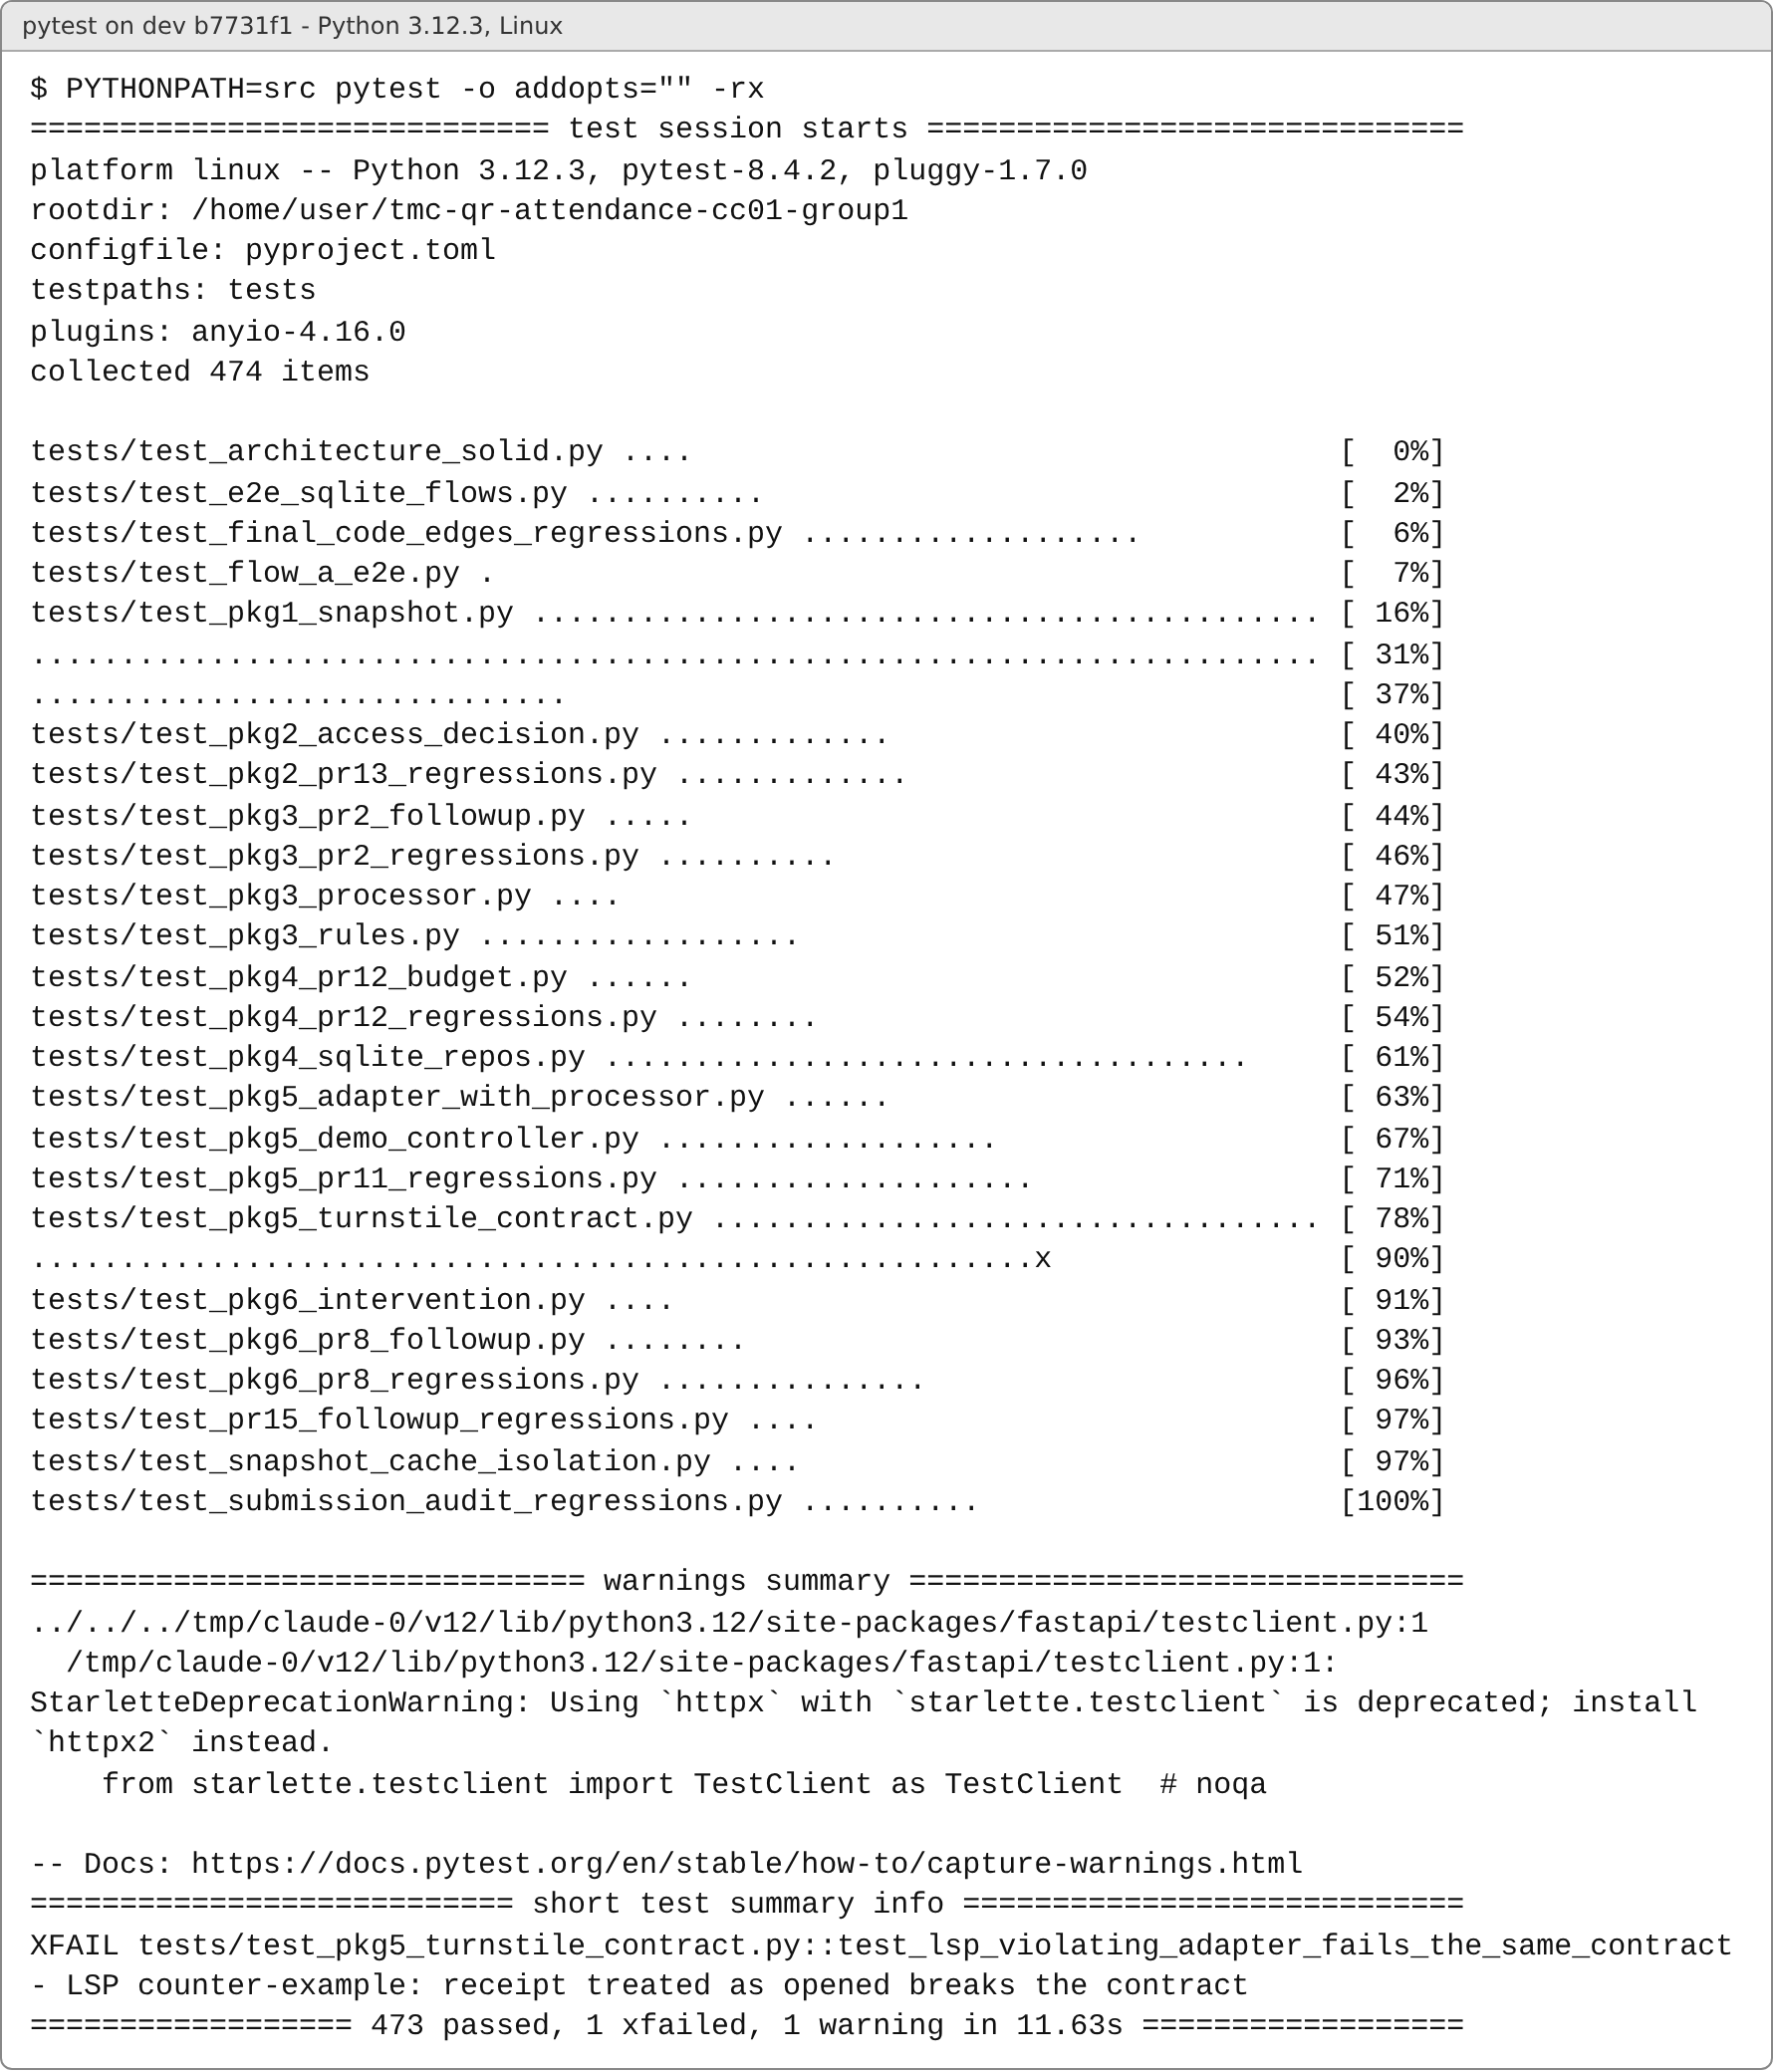
\includegraphics[width=0.92\linewidth]{figure/figure-9-8-pytest-run.png}

\vspace{6pt}
\textbf{Figure 9.8. Output of the Test Suite: 473 Passed and 1 Expected Failure}
\phantomsection\addcontentsline{lof}{figure}{\protect\numberline{9.8}Output of the Test Suite}
\end{minipage}

\vspace{10pt}

The ten tests in \code{test_e2e_sqlite_flows.py} are the closest our automated tests get to a real run. Each one builds the whole application with \code{create_app()} on a real SQLite file, signs QR codes with Ed25519, talks to it over HTTP, and then opens the file with a separate connection to check what was really committed. For Flow A they show that:

\begin{itemize}[leftmargin=36pt, itemsep=2pt, topsep=4pt, parsep=2pt]
  \item a full cycle where the controller sends every signal twice still gives one openGate, one attendance record, and one closeGate;
  \item a copied QR code scanned on another lane is rejected as a replay, and a malformed token or a suspended employee is rejected before any command;
  \item with a watermark age of 300 seconds the scan is accepted in DEGRADED mode and the attendance record carries the degraded flag, and at 1800 seconds the scan is CANNOT\_PROCESS;
  \item an UNDETERMINED opening becomes PENDING\_RECONCILIATION without a second openGate, and the lane and the token stay held; a CONTROLLER\_ERROR releases the lane. The rule that the controller is queried exactly once is checked separately in \code{test_pkg5_adapter_with_processor.py};
  \item the stored state is still there after the application is restarted on the same file.
\end{itemize}

For Flow B they show that a request without a guard session gets HTTP 401, that an assisted opening stores the support case once and creates no attendance, and that an emergency hold makes new scans return LANE\_BUSY until the reset, after which LANE\_CLEAR closes the gate. One rule has no end-to-end test: a PASSAGE that arrives after the 15-second window. It is checked only at processor level (\code{test_pkg3_rules.py}) and for storage (\code{test_pkg4_sqlite_repos.py}).


We also ran the four demo scenarios of the README through FastAPI's TestClient on a SQLite file, and all of them gave the expected results. The three manual runs in Section 9.5 (Figures 9.5 to 9.7) were done on a real Uvicorn server with a SQLite file. Table 9.8 lists what each part of them shows. The order of the writes before openGate and the single closeGate call are checked by the tests in Table 9.6, not by this run. The scripts are kept in \code{report/evidence/}: \code{run_demo.py}, which produced the figures, and bash versions of the same runs together with the captured output and Uvicorn logs of an earlier run, which differ from the figures only in generated ids and times. Clicking through the Swagger page during the presentation is still a manual step.

\begin{longtable}{|>{\raggedright\arraybackslash}p{36pt}|>{\raggedright\arraybackslash}p{124pt}|>{\raggedright\arraybackslash}p{134pt}|>{\raggedright\arraybackslash}p{104pt}|}
\hline
\multicolumn{1}{|>{\columncolor{tableheader}\centering\arraybackslash}p{36pt}|}{\textbf{Figure, part}} & \multicolumn{1}{>{\columncolor{tableheader}\centering\arraybackslash}p{124pt}|}{\textbf{What we sent}} & \multicolumn{1}{>{\columncolor{tableheader}\centering\arraybackslash}p{134pt}|}{\textbf{What we observed}} & \multicolumn{1}{>{\columncolor{tableheader}\centering\arraybackslash}p{104pt}|}{\textbf{What it shows}} \\
\hline
\endhead
\multicolumn{4}{c}{\rule{0pt}{20pt}\normalsize\textbf{Table 9.8. Manual Runs on Uvicorn with a SQLite File}} \\
\endlastfoot
9.5 (a) & Scan S-1 with a fresh QR code on LANE-BD-01 & OPENED, OPEN\_CONFIRMED, and a commandId & Confirmed opening for a valid scan \\
\hline
9.5 (b) & Scan S-2 with the same code on LANE-BD-02 & REJECTED, QR\_TOKEN\_\allowbreak REPLAY\_\allowbreak DETECTED, no command & Single-use token claim (ADR-11) \\
\hline
9.5 (c) & PASSAGE PE-1 twice, then LANE\_CLEAR twice, for the commandId of S-1 & Each request answered with HTTP 200; this alone does not prove deduplication & -- \\*
\hline\noalign{\nobreak}
9.5 (d) & Read the database file with a separate connection & One attendance record (S-1, PE-1, EMP-001, ENTRY), one passage event, one OPEN and one CLOSE command & Repeated signals leave one attendance record and one persisted CLOSE command \\
\hline
9.6 (a) & Watermark age 300 s, then scan S-10 & DEGRADED; S-10 OPENED with the degraded flag; its attendance record is flagged & Bounded degraded mode, flagged for review (I-10) \\
\hline
9.6 (b) & Watermark age 1800 s, then scan S-11 & CANNOT\_PROCESS, no command & No automatic scan from 30 minutes (I-10) \\
\hline
9.6 (c), (d) & openGate times out, status query undetermined; scan S-12, then S-13 on the same lane & S-12 PENDING\_RECONCILIATION with one stored OPEN command, outcome UNDETERMINED; S-13 LANE\_BUSY & Uncertain opening stays pending and keeps the lane held (I-03) \\
\hline
9.7 (a) & Assisted opening without X-Guard-Session & HTTP 401 & Guard comes from the session \\
\hline
9.7 (b) & The same assisted opening twice with a session & Same commandId both times; one stored OPEN command for case-001 & A repeated request reuses the stored command \\
\hline
9.7 (c) & PASSAGE PE-30 at once, then LANE\_CLEAR, for the assisted commandId & HTTP 200 for both; CLOSE command stored for case-001 & -- \\
\hline
9.7 (d), (e) & Emergency release, scan, reset, LANE\_CLEAR, scan & EMERGENCY\_HOLD, LANE\_BUSY, RESET\_CONFIRMED, CLOSED, then OPENED & Emergency hold blocks scans until reset and close \\
\hline
9.7 (f) & Read the database file & Two support cases; PE-30 stored with no review reason; no attendance record & A timely passage after an assisted opening creates no attendance by itself \\
\hline
\end{longtable}
\phantomsection\addcontentsline{lot}{table}{\protect\numberline{9.8}Manual Runs on Uvicorn with a SQLite File}

Table 9.8 only states what can be seen in the HTTP answers and in the database file. A stored command row does not prove how often the adapter was called, and the demo server does not print the command log of the simulated controller. The rule that an uncertain OPEN is not sent again, and that a repeated assisted request does not reach the controller a second time, is therefore checked by tests that count the commands the simulated controller received. In \code{test_e2e_sqlite_flows.py} these are \code{test_flow_a_undetermined_open_is_queried_once_and_never_resent} and \code{test_flow_b_assisted_open_records_case_without_attendance}, and the third is \code{test_resending_identical_support_case_is_idempotent} in \code{test_pkg6_pr8_regressions.py}.

\Needspace{9\baselineskip}
\subsection*{9.8. What the Prototype Does Not Show}

\phantomsection
\addcontentsline{toc}{subsection}{9.8. What the Prototype Does Not Show}

Passing tests do not close the open issues listed in Section 10.2. The simulated controller answers commands the way I-01 and I-03 assume, and the PASSAGE and LANE\_CLEAR signals of I-05 are sent by the tests and scripts, so the runs show that Gate Core handles those signals correctly, but not that a real controller sends them. The tests check how the 2-second budget is shared out using a test clock; they do not measure the response time on factory hardware with a real kiosk and controller. There is also a gap in the budget itself. The prototype starts a 2,000 ms processing budget when processScan begins, because the HTTP route does not pass a kiosk deadline. This budget does not reserve the kiosk, network, and display time allocated in Table 5.4. Meeting NFR-01 requires budgeting those stages together and measuring from QR reading to result display. SQLite has no standby, so the synchronous replication and the failover rules of Section 5.6 are not tested either.

Synchronization is only partly there. IFactoryUpdates applies snapshot changes and reads the local outbox, but without Site Sync or a central application we drive degraded mode by setting the age of the access data by hand. Finally, the guard session and the authorization checks are demo stubs, and the QR private key is created in the same process as the factory code, which the target design does not allow.


\Needspace{9\baselineskip}
\subsection*{9.9. Source Code}

\phantomsection
\addcontentsline{toc}{subsection}{9.9. Source Code}

The implementation, the automated tests, and the LaTeX source of this report are available at

\begin{center}
{\small\url{https://github.com/Khoavan1406-hub/tmc-qr-attendance-cc01-group1}}
\end{center}

The Python package is in \code{src/tmc_gate/}, the tests are in \code{tests/}, and the report source is in \code{report/}. The \code{README.md} file at the root of the repository explains how to install the dependencies, run the test suite, and start the demo, while \code{ARCHITECTURE_RULES.md} records the rules we followed when writing the code, such as the allowed import directions and the gate thresholds. The architectural decisions themselves are not kept as separate files in the repository; they are documented in Chapter 6. All work was merged into the \texttt{dev} branch through pull requests. The code in \code{src/} and \code{tests/} has not changed since commit 5bd6721, which is the commit behind the test results in Section 9.7.
